% !TEX program = xelatex
\documentclass[10pt,aspectratio=169]{beamer}
\makeatletter
\def\@makefnmark{}
\makeatletter
\usepackage{amsthm,amsmath,amssymb,braket,fontspec,unicode-math,bbding}
\usepackage[absolute,overlay]{textpos}
\usetheme[numbering=none]{focus}
\setbeamercolor{footnote}{fg=azure}
\setbeamerfont{footnote}{size=\tiny,series=\bfseries}
\setbeamerfont{alerted text}{series=\bfseries}

\setmathfont{Latin Modern Math}[range={frak,\bigcap,\bigcup}]

\usepackage[backend=bibtex,url=false,doi=false,maxcitenames=1, style=authoryear]{biblatex}
\bibliography{bib}
\AtBeginBibliography{\scriptsize}

\newcommand{\focus}[1]{\textcolor{red}{\bf{#1}}}
\AtBeginSection[]{}
\definecolor{red}{HTML}{CC0000}
\definecolor{lred}{HTML}{e24a33}
\definecolor{bgreen}{HTML}{006A4E}
\definecolor{azure}{HTML}{007fff}
\newcommand{\alertb}[1]{\color{azure}\alert{#1}}
\setbeamertemplate{bibliography item}[triangle]

\graphicspath{{./figures/}}

%\AtBeginSection[]{
%  \vfill
%  \centering
%  \begin{beamercolorbox}[sep=20pt,rounded=true,center]{frametitle}
%    \usebeamerfont{title}\insertsectionhead\par%
%  \end{beamercolorbox}
%  \vfill
%}
\title{\LARGE Emergence in correlated fermions: From impurity models to the bulk}

\author{\textbf{Abhirup Mukherjee}\\\alert{RPC Presentation 2022-2023}}
\institute{\textbf{Emergent Phenomena in Quantum Matter} Group\\
Department of Physical Sciences, IISER Kolkata}

\date{July 11, 2023}
\begin{document}

\centering

\begin{frame}
\maketitle
\begin{textblock*}{0.13\textwidth}(13.5cm, 4.3cm)
	\centering

	
\includegraphics[width=\textwidth]{epqm_logo_mod.jpeg}\\
	\vspace*{\fill}
	
\includegraphics[width=\textwidth]{dps_logo.jpeg}
\end{textblock*}
\end{frame}

\begin{frame}{}
\hspace*{\fill}
\begin{minipage}{0.1\textwidth}
	
\includegraphics[width=\textwidth]{epqm_logo_mod.jpeg}
\end{minipage}
\begin{minipage}{0.25\textwidth}
	\centering
	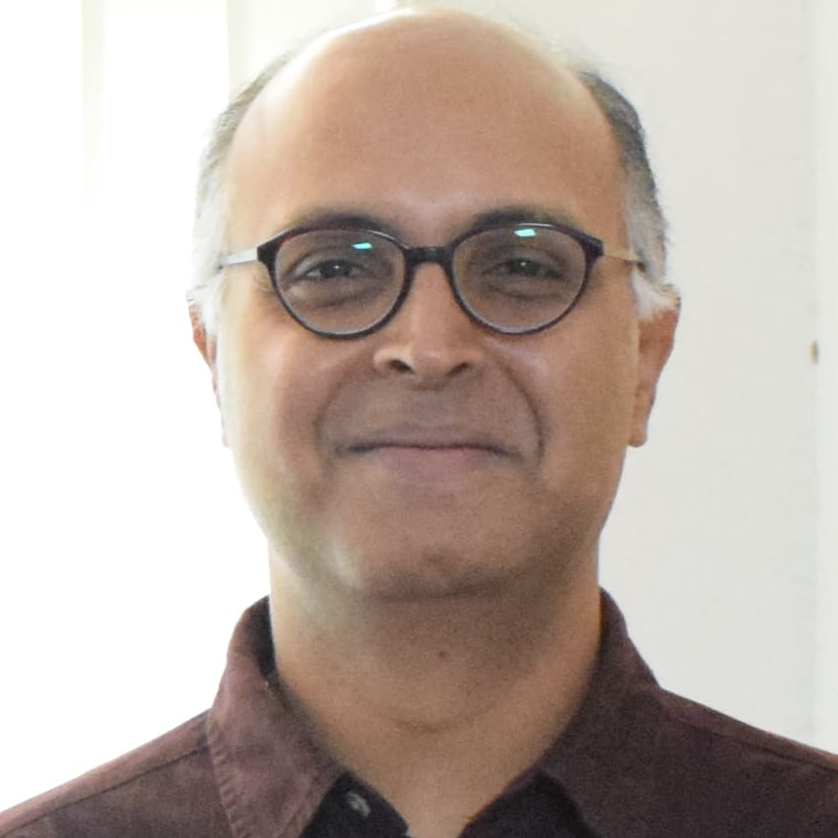
\includegraphics[width=0.6\textwidth]{slal.jpg}\\
	\footnotesize{{\bf Siddhartha Lal}\\
	}
\end{minipage}
\begin{minipage}{0.25\textwidth}
	\centering
	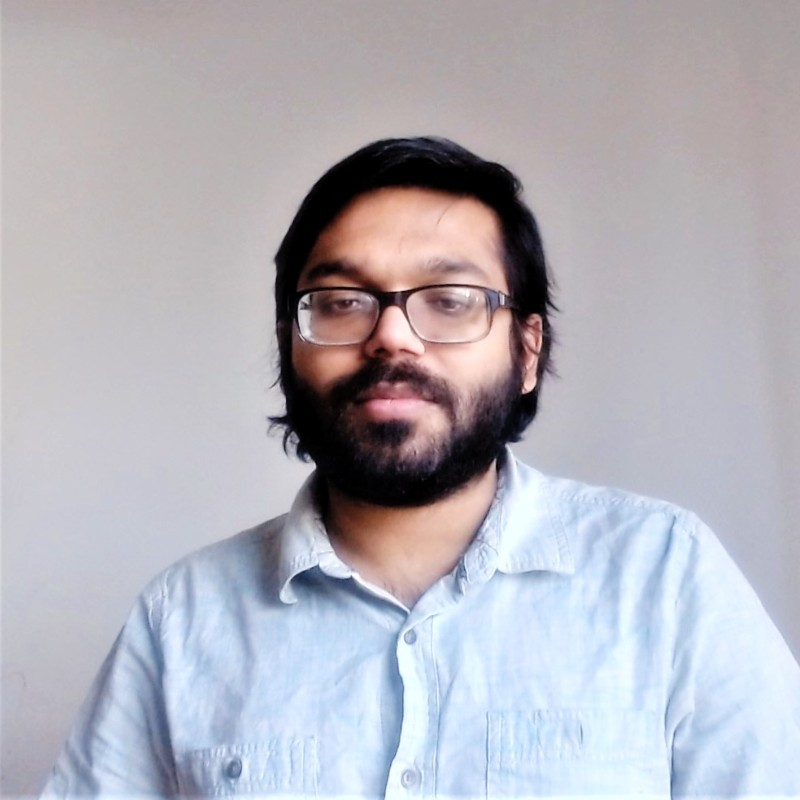
\includegraphics[width=0.6\textwidth]{amukherjee.jpg}\\
	\footnotesize{{\bf Anirban Mukherjee}\\
	}
\end{minipage}
\begin{minipage}{0.25\textwidth}
	\centering
	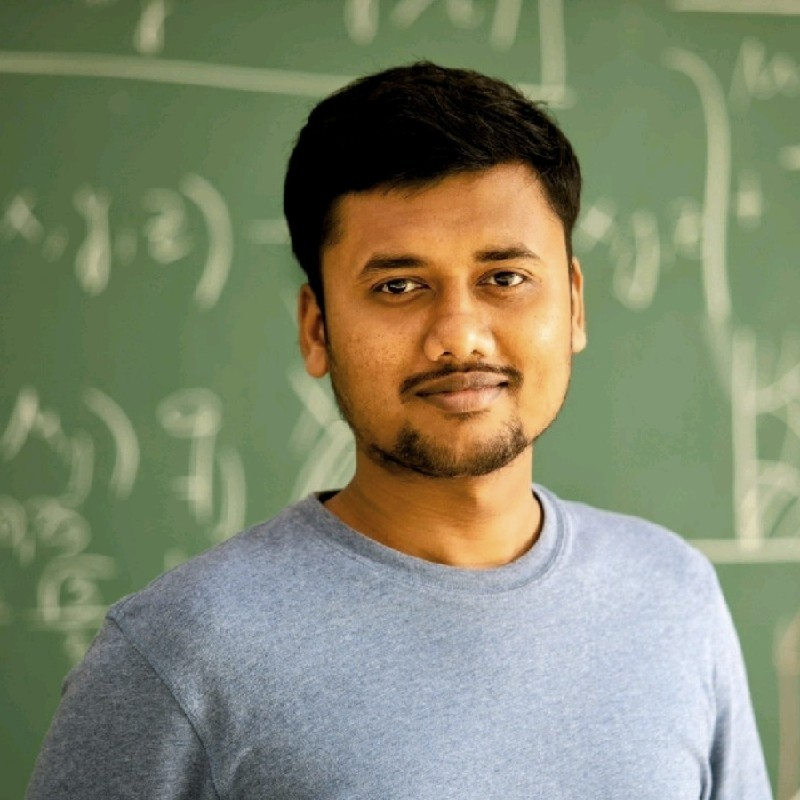
\includegraphics[width=0.6\textwidth]{spatra.jpeg}\\
	\footnotesize{{\bf Siddhartha Patra}\\
	}
\end{minipage}
\begin{minipage}{0.1\textwidth}
	
\includegraphics[width=\textwidth]{dps_logo.jpeg}
\end{minipage}
\hspace*{\fill}
\\
\vspace*{\fill}
\begin{minipage}{0.18\textwidth}

\includegraphics[width=\textwidth]{IISER-K.png}
\end{minipage}
\hspace*{\fill}
\begin{minipage}{0.6\textwidth}
\centering
\alert{$\sim\sim\sim\sim\sim\sim\sim\sim\sim\sim\sim\sim\sim\sim\sim$ }\\
\alert{A huge thanks to all my collaborators! }\\[10pt]
\alert{Thanks to IISER K and SERB for financial support.}\\
\alert{$\sim\sim\sim\sim\sim\sim\sim\sim\sim\sim\sim\sim\sim\sim\sim$ }\\
\end{minipage}
\hspace*{\fill}
\begin{minipage}{0.18\textwidth}

\includegraphics[width=\textwidth]{SERB.png}
\end{minipage}
\vspace*{\fill}

\hspace*{\fill}
\begin{minipage}{0.1\textwidth}
	
\includegraphics[width=\textwidth]{IITKGP.png}\\
\end{minipage}
\hspace*{\fill}
\begin{minipage}{0.3\textwidth}
	\centering
	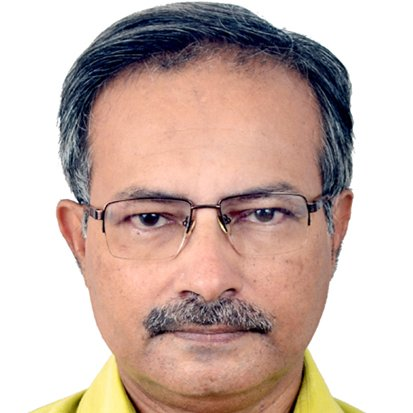
\includegraphics[width=0.45\textwidth]{arghya.jpg}\\
	\footnotesize{{\bf Arghya Taraphder}\\
	IIT Kharagpur}
\end{minipage}
\hspace*{\fill}
\begin{minipage}{0.3\textwidth}
	\centering
	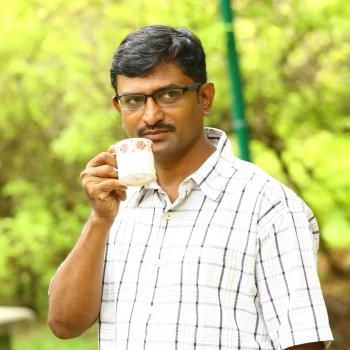
\includegraphics[width=0.45\textwidth]{nsv.jpeg}\\
	\footnotesize{{\bf N. S. Vidhyadhiraja}\\
	JNCASR Bangalore}
\end{minipage}
\hspace*{\fill}
\begin{minipage}{0.1\textwidth}
	
\includegraphics[width=\textwidth]{JNCASR.png}\\
\end{minipage}
\hspace*{\fill}

\end{frame}

\section{List of publications, preprints and ongoing projects}
\subsection{~}

\begin{frame}{List of publications, preprints and ongoing projects}
\only<1-2>{
\begin{itemize}
	\item[\Checkmark] \onslide<1->{\only<1>{Unveiling the Kondo cloud: Unitary renormalization-group study of the Kondo model.\\[5pt] } 2022 \alert{Phys. Rev. B} 105, 085119.\\[5pt] A Mukherjee, \alert{Abhirup Mukherjee}, N. S. Vidhyadhiraja, A. Taraphder, and S Lal\\[10pt]}
	\item[\Checkmark] \onslide<1->{\only<1>{Frustration shapes multi-channel Kondo physics: a star graph perspective.\\[5pt] } 2023 \alert{J. Phys.: Condens. Matter} 35 315601. \\[5pt] S Patra, \alert{Abhirup Mukherjee}, A Mukherjee, N S Vidhyadhiraja, A Taraphder and S Lal\\[10pt]
	}
	\item \onslide<2->{\only<2>{Kondo frustration via charge fluctuations: a route to Mott localisation.\\[5pt] } 2023 \alert{arXiv:2302.02328}. under review at New Journal of Physics.\\[5pt] \alert{Abhirup Mukherjee}, N. S. Vidhyadhiraja, A. Taraphder, S Lal\\[10pt]}
	\item \onslide<2->{\only<2>{Holographic entanglement renormalisation for fermionic quantum matter: geometrical and topological aspects.\\[5pt]} 2023 \alert{arXiv:2302.10590}. under review at Journal of HEP.\\[5pt] \alert{Abhirup Mukherjee}, S Patra, S Lal\\[10pt]
	}
\end{itemize}
}
\only<3>{
\begin{minipage}{0.53\textwidth}
\begin{itemize}
	\item[\Checkmark] 2022 \alert{Phys. Rev. B} 105, 085119.\\[5pt] A Mukherjee, \alert{Abhirup Mukherjee}, N. S. Vidhyadhiraja, A. Taraphder, and S Lal
	\item[\Checkmark] 2023 \alert{J. Phys.: Condens. Matter} 35 315601.\\[5pt] S Patra, \alert{Abhirup Mukherjee}, A Mukherjee, N S Vidhyadhiraja, A Taraphder and S Lal
\end{itemize}
\end{minipage}
\begin{minipage}{0.45\textwidth}
\begin{itemize}
	\item 2023 \alert{arXiv:2302.02328}.\\[5pt] \alert{Abhirup Mukherjee}, N. S. Vidhyadhiraja, A. Taraphder, S Lal\\[5pt]
	\item 2023 \alert{arXiv:2302.10590}.\\[5pt] \alert{Abhirup Mukherjee}, S Patra, S Lal
\end{itemize}
\end{minipage}
\vspace*{\fill}
\begin{itemize}
	\item \onslide<3>{We are currently finishing the development of a new auxiliary model-based approach to studying correlated systems in the bulk.\\[10pt]}
	\item \onslide<3>{We have begun work on a project that aims to provide new insights on the plateau-to-plateau transition in integer quantum hall systems.
	}
\end{itemize}
}
\end{frame}

\begin{frame}{How to explain the resistance minimum \& eventual saturation?}
\footcite{wilson1975,andrei_1980,Wiegmann_1981,affleck1995conformal}
Breakdown of perturbation theory indicates a \alert{change in ground state}!\\[10pt]
Obtaining \(T=0\) ground state requires more \alert{powerful  methods}\\[10pt]

\begin{minipage}{0.2\textwidth}
\centering
Numerical RG\\[10pt]
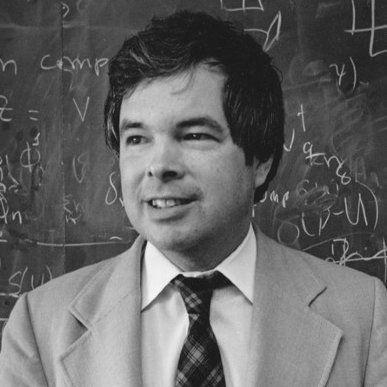
\includegraphics[width=0.5\textwidth]{wilson.jpg}\\
\footnotesize{(K. G. Wilson)}
\end{minipage}
\begin{minipage}{0.2\textwidth}
\centering
Bethe ansatz\\[10pt]
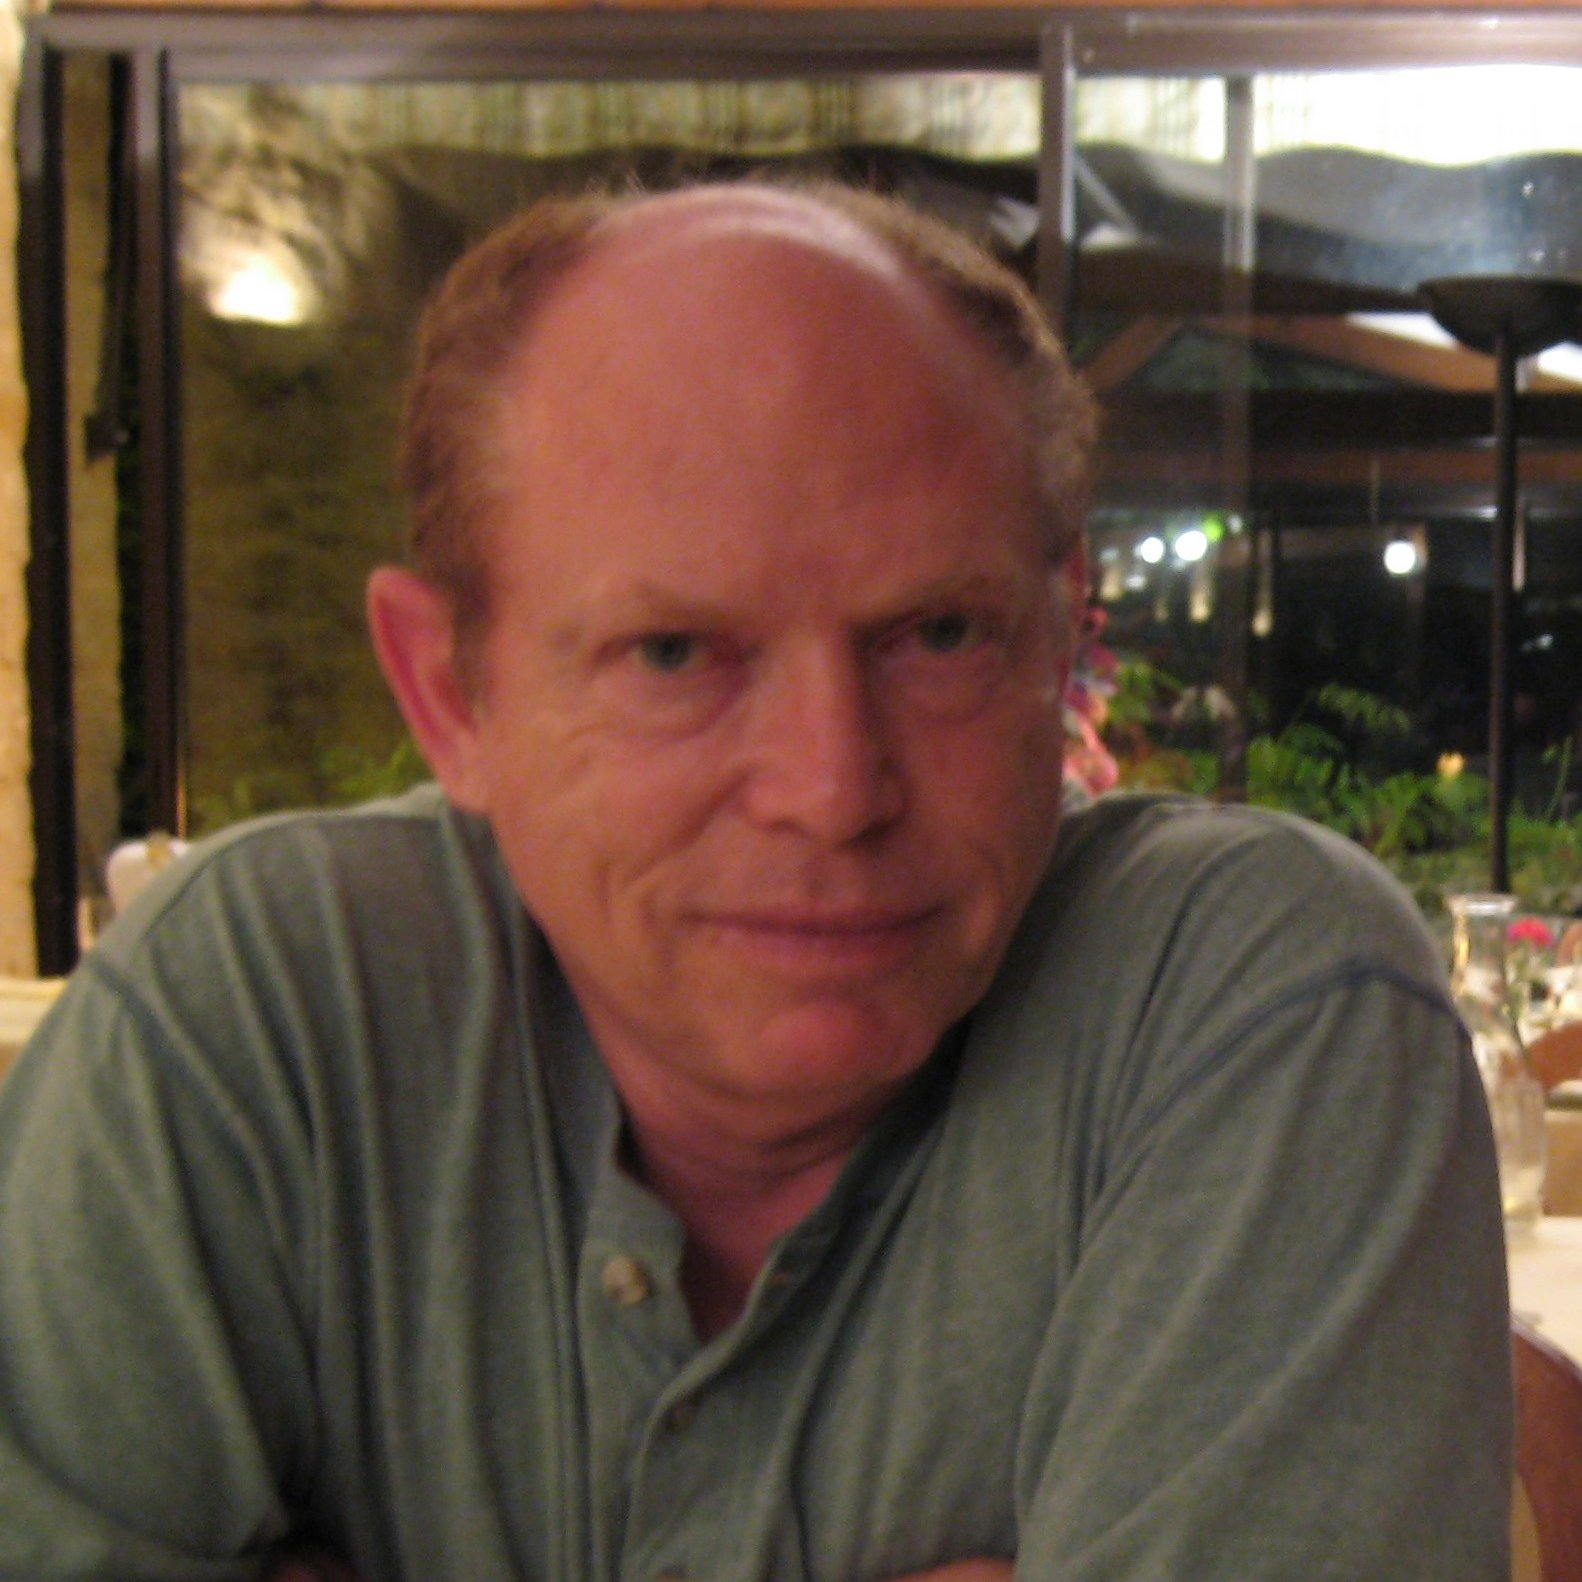
\includegraphics[width=0.5\textwidth]{AndreiN.jpg}\\
\footnotesize{(Natan Andrei)}
\end{minipage}
\begin{minipage}{0.2\textwidth}
\centering
Conf. field theory\\[10pt]
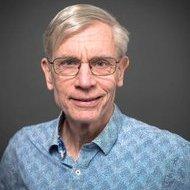
\includegraphics[width=0.5\textwidth]{affleck.jpg}\\
\footnotesize{(Ian Affleck)}
\end{minipage}
\begin{minipage}{0.38\textwidth}
\begin{itemize}
	\item impurity becomes \alert{strongly coupled} at low temperatures
	\item local moment crosses over into \alert{nonmagnetic} singlet
\end{itemize}
\end{minipage}

\vspace*{\fill}
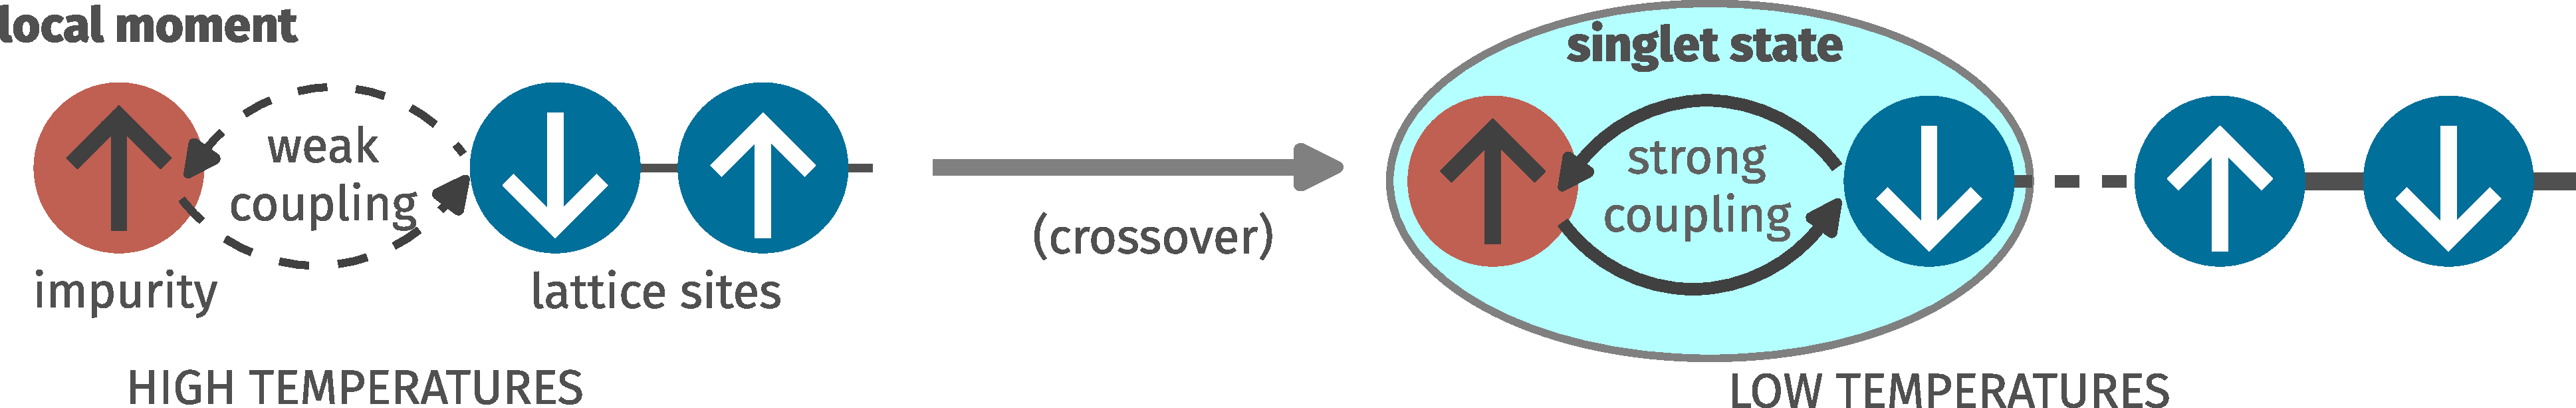
\includegraphics[width=0.9\textwidth]{crossover.pdf}\\

\end{frame}

\section{Some important questions}
\begin{frame}{Some important questions}
\begin{minipage}{0.45\textwidth}
	How do we describe the dynamics of the electrons that screen the impurity (the so-called \alert{Kondo cloud})?\\
	\footnotesize{[Mukherjee et al 2023 Phys. Rev. B 105, 085119]}
\end{minipage}
\hspace*{\fill}
\begin{minipage}{0.45\textwidth}
	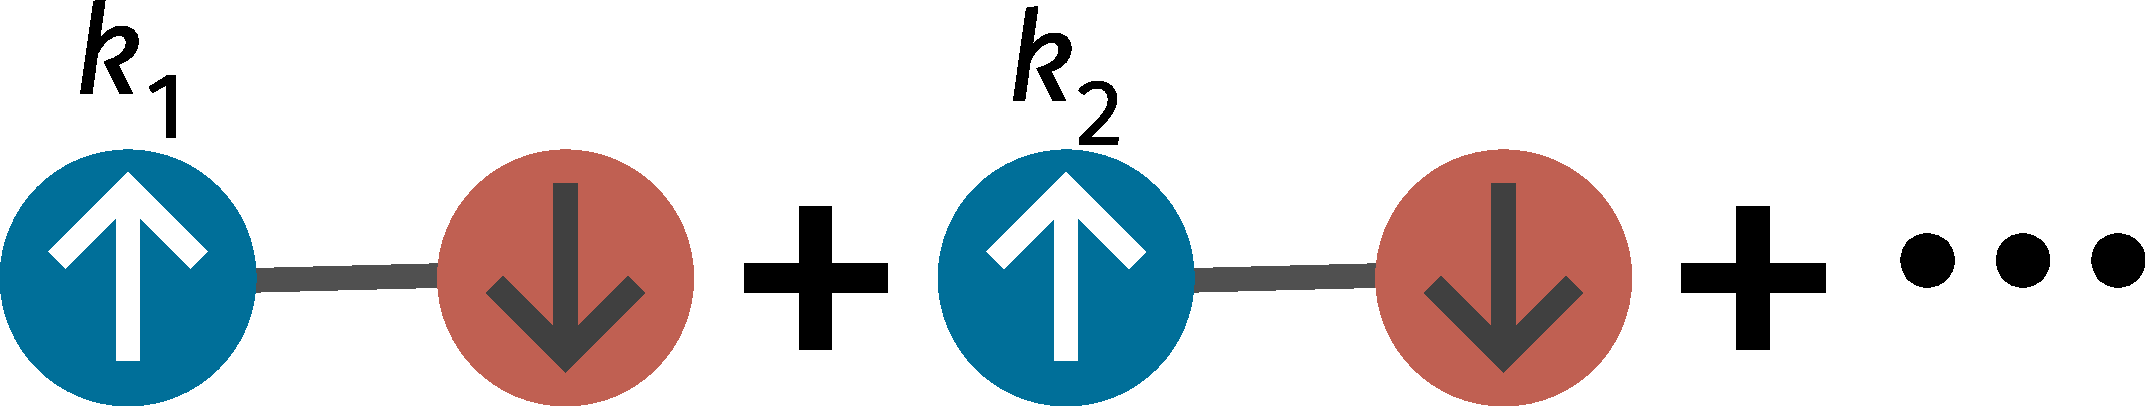
\includegraphics[width=0.9\textwidth]{kondocloud.pdf}
\end{minipage}
\vspace*{\fill}

\begin{minipage}{0.45\textwidth}
	
\includegraphics[width=0.9\textwidth]{distortsinglet.pdf}
\end{minipage}
\hspace*{\fill}
\begin{minipage}{0.45\textwidth}
	What kind of physics can \alert{disturb the Kondo screening} effect and distort the singlet state?\\
	\footnotesize{[Patra et al 2023 J. Phys.: Condens. Matter 35 315601]}
\end{minipage}
\vspace*{\fill}

\begin{minipage}{0.45\textwidth}
	What is the simplest impurity model that completely destroys the Kondo effect and leads to a \alert{phase transition}?\\
	\footnotesize{[Mukherjee et al 2023 arXiv:2302.02328]}
\end{minipage}
\hspace*{\fill}
\begin{minipage}{0.45\textwidth}
	
\includegraphics[width=0.9\textwidth]{kondobreakdown.pdf}
\end{minipage}
\end{frame}

\section{The single-channel Kondo problem:\\ Anatomy of the Kondo cloud\vspace*{20pt}}
\begin{textblock*}{\textwidth}(1cm, 3.5cm)

\includegraphics[width=\textwidth]{kondocloud_prb.pdf}\\
\end{textblock*}
\subsection{~}

\begin{frame}{Effective Hamiltonian for the Kondo cloud}
\footcite{anirban_kondo,anirbanurg1,anirbanurg2}
We first applied the \alert{unitary RG} to obtain a low energy fixed point theory.\\[10pt]
To obtain a theory for the Kondo cloud, we \alert{trace out impurity} from fixed point Hamiltonian.
\vspace*{\fill}

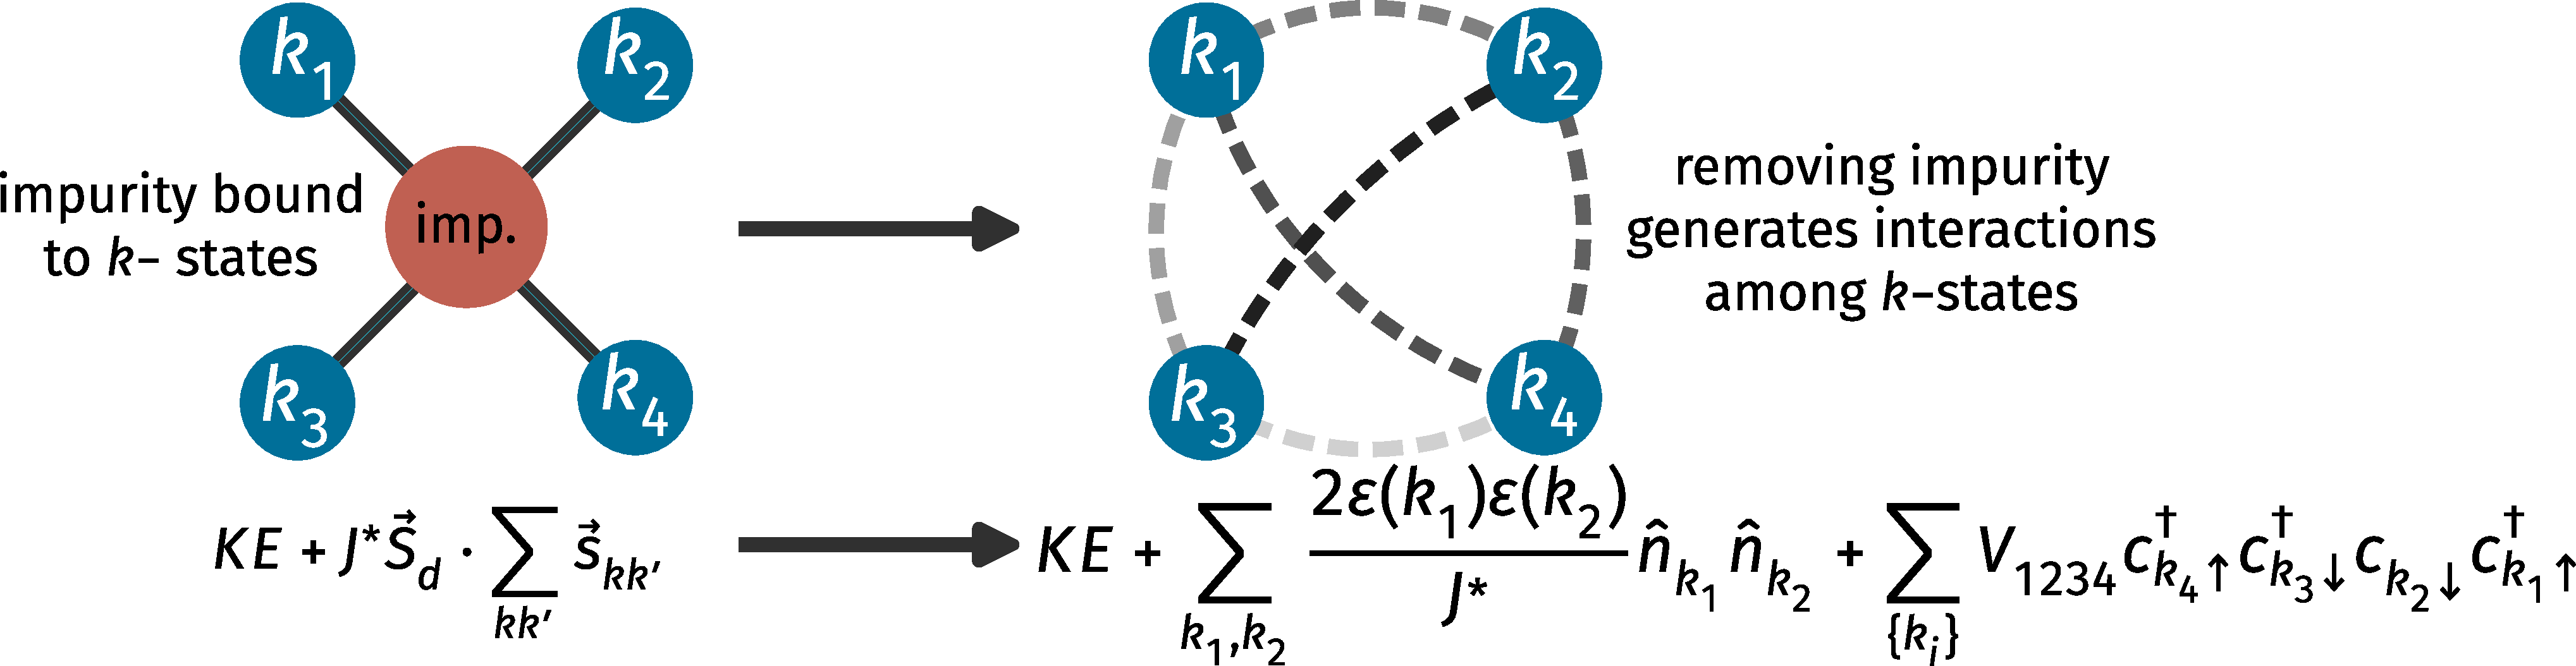
\includegraphics[width=\textwidth]{KondoCloud.pdf}

\vspace*{\fill}
\begin{itemize}
	\item all-to-all interactions between momentum states, \alert{large entanglement}
	\item 2-particle interaction terms \alert{not} present in Fermi liquid, are \alert{responsible for screening}
\end{itemize}

\end{frame}

\begin{frame}{Quantifying entanglement within the Kondo cloud}
\footcite{anirban_kondo}
In order to demonstrate formation of Kondo cloud, we study the \alert{variation of entanglement} and correlations under RG transformations.

\vspace*{\fill}
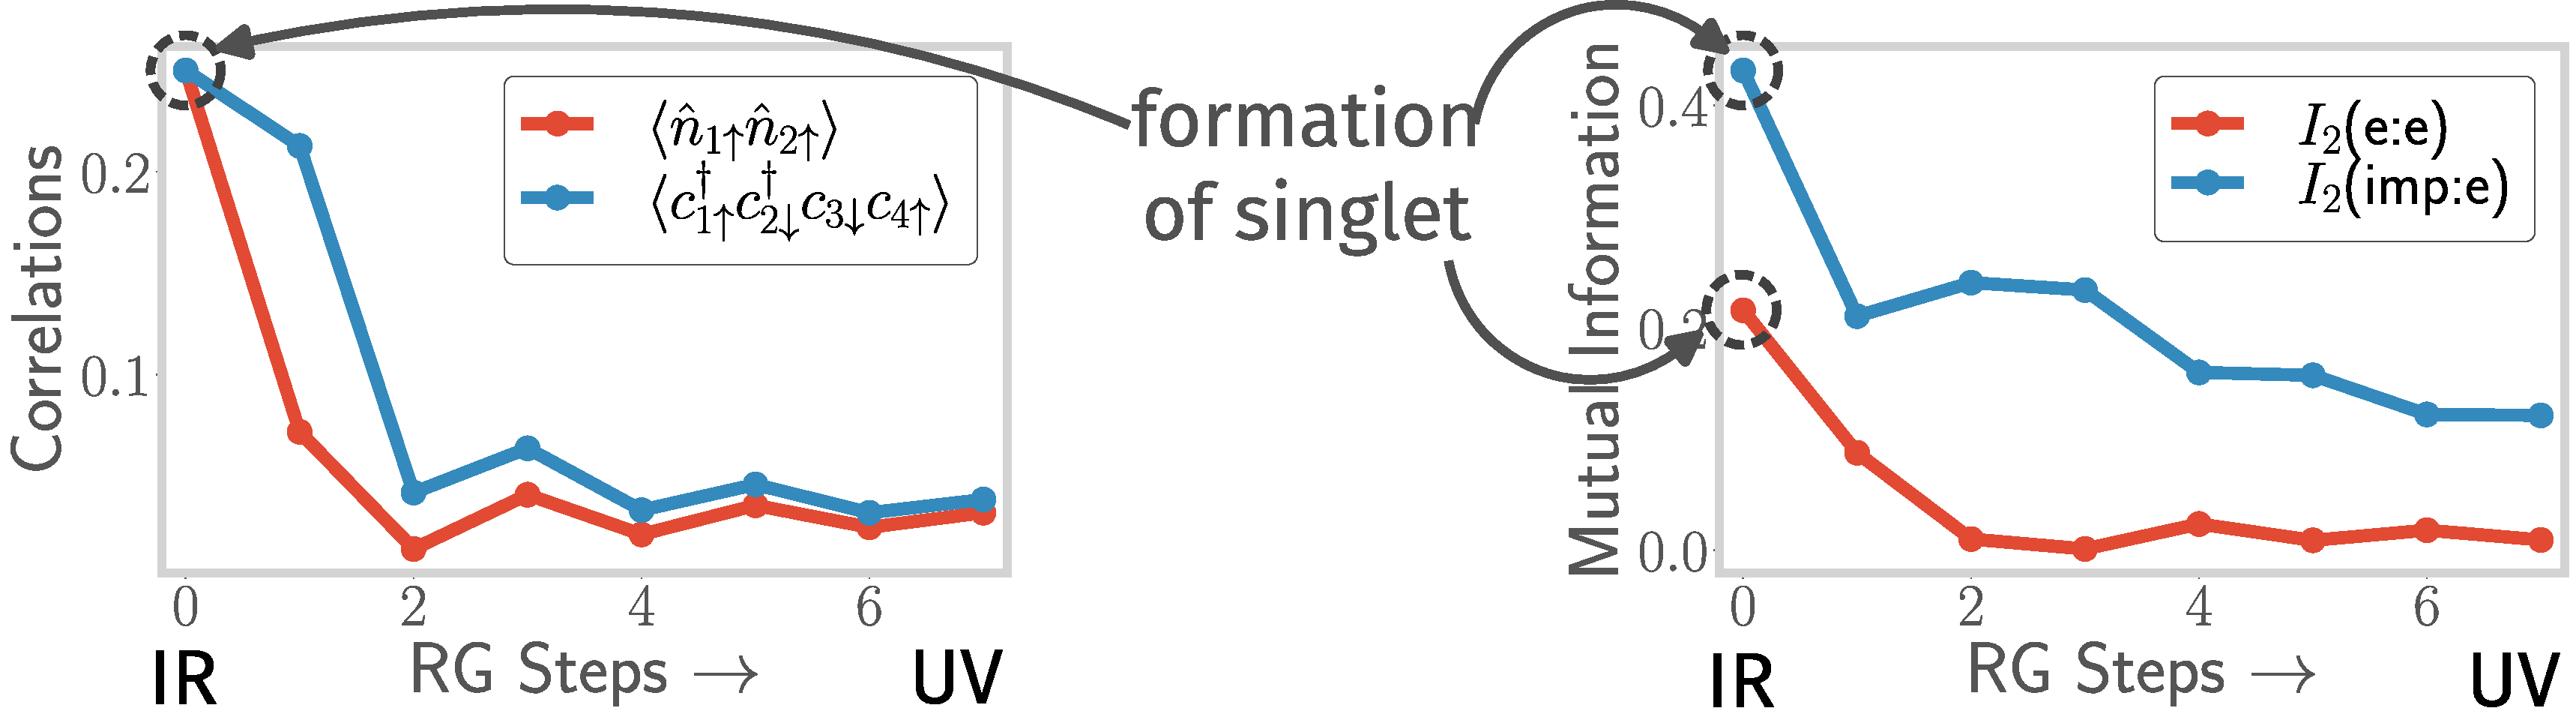
\includegraphics[width=\textwidth]{kondoRevRG.pdf}

\vspace*{\fill}
\begin{itemize}
	\item Both entanglement and \(k-\)space correlations \alert{increase} as RG proceeds from UV to IR.\\[10pt]
	\item This shows the formation of the \alert{Kondo singlet} and the growth of two-particle correlations in the \alert{Kondo cloud}.
\end{itemize}
\end{frame}

\section{Distorting the Kondo singlet:\\ The multi-channel Kondo Problem\vspace*{20pt}}
\begin{textblock*}{\textwidth}(1cm, 3.5cm)

\includegraphics[width=0.8\textwidth]{MCKJPCM.pdf}
\end{textblock*}
\subsection{~}

\begin{frame}{What is the multichannel Kondo problem?}
\footcite{Noz_blandin_1980,affleck1993exact,emery_kivelson,andrei_destri_1984}
\begin{minipage}{0.39\textwidth}
Single impurity interacting with \alert{multiple channels} in the bath
\[H_\text{Kondo} = KE_\text{bath} + \sum_{l}J_l \vec{S}_\text{imp}\cdot\vec{s}^{(l)}\]
\end{minipage}
\hspace*{\fill}
\begin{minipage}{0.59\textwidth}
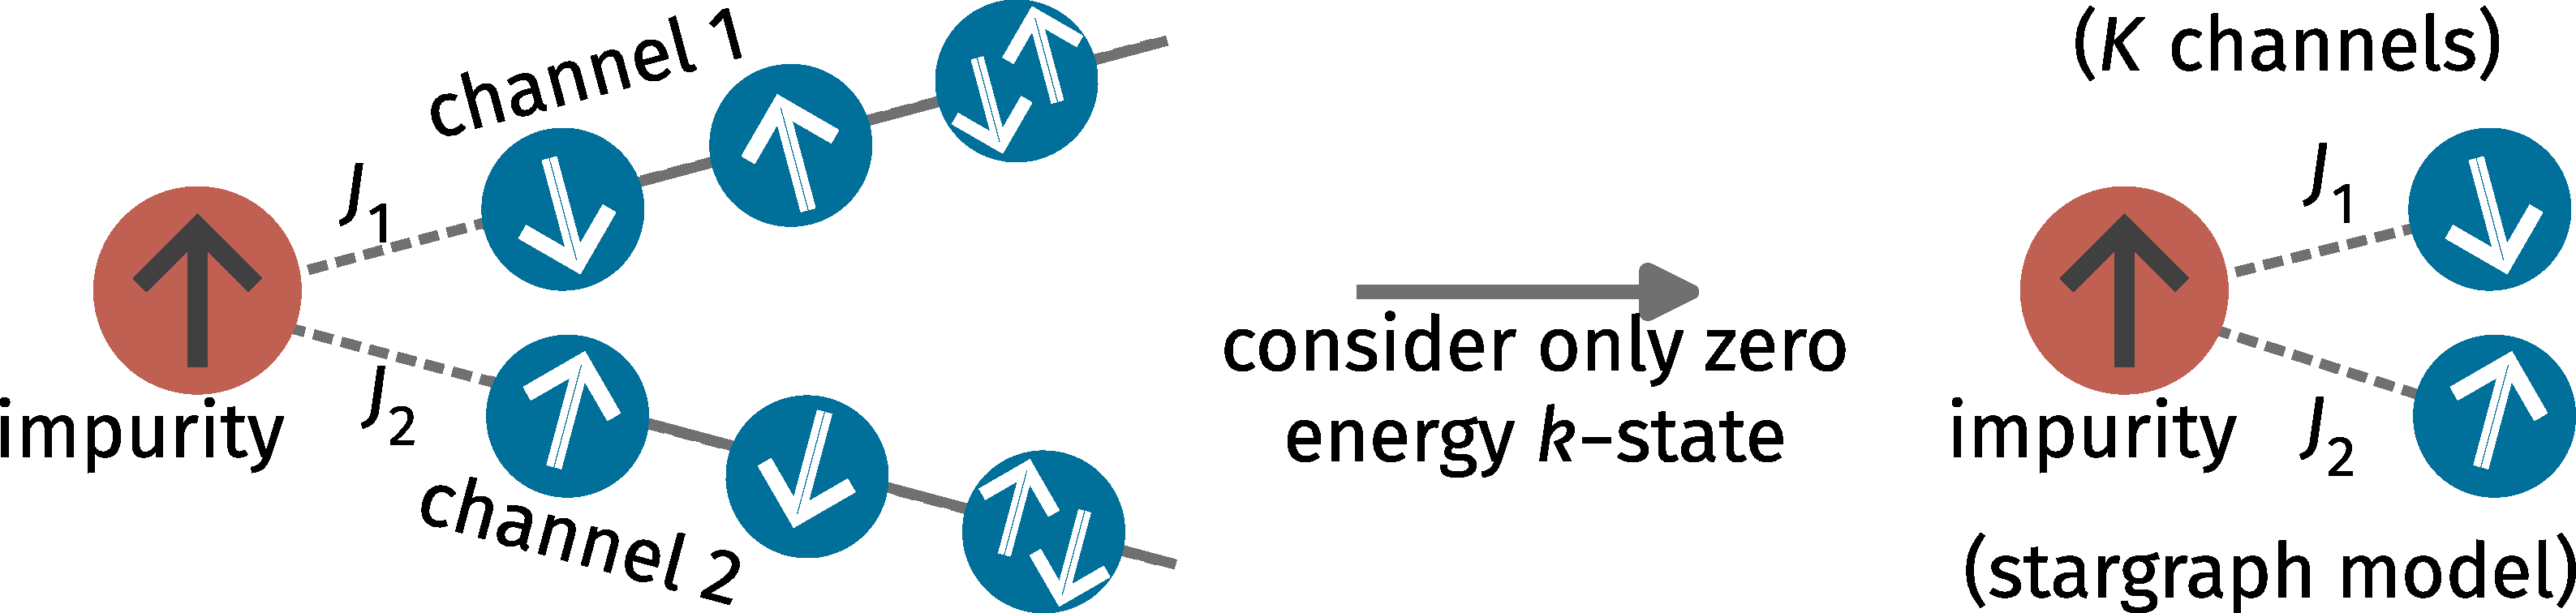
\includegraphics[width=\textwidth]{MCKM_zeroB.pdf}
\end{minipage}\\[10pt]
Known to display divergent \(T=0\) impurity susceptibility (incomplete screening), and orthogonality catastrophe, \alert{non-Fermi liquid} excitations.\\[10pt]
\begin{minipage}{0.64\textwidth}
Zero bandwidth limit is (analytically) solvable: \(\left\{\ket{S_\text{tot}^z}\right\}\)\\
\begin{itemize}
	\item Ground state degeneracy for \(K > 1\) explains \alert{orthogonality catastrophe}\\[5pt]
\item \(S_\text{tot}^z \neq 0\) in ground states shows incomplete screening\\[5pt]
\item Excitations shows \alert{non-Fermi liquid} physics in the form of inter-channel scattering.
\end{itemize}
\end{minipage}
\begin{minipage}{0.35\textwidth}
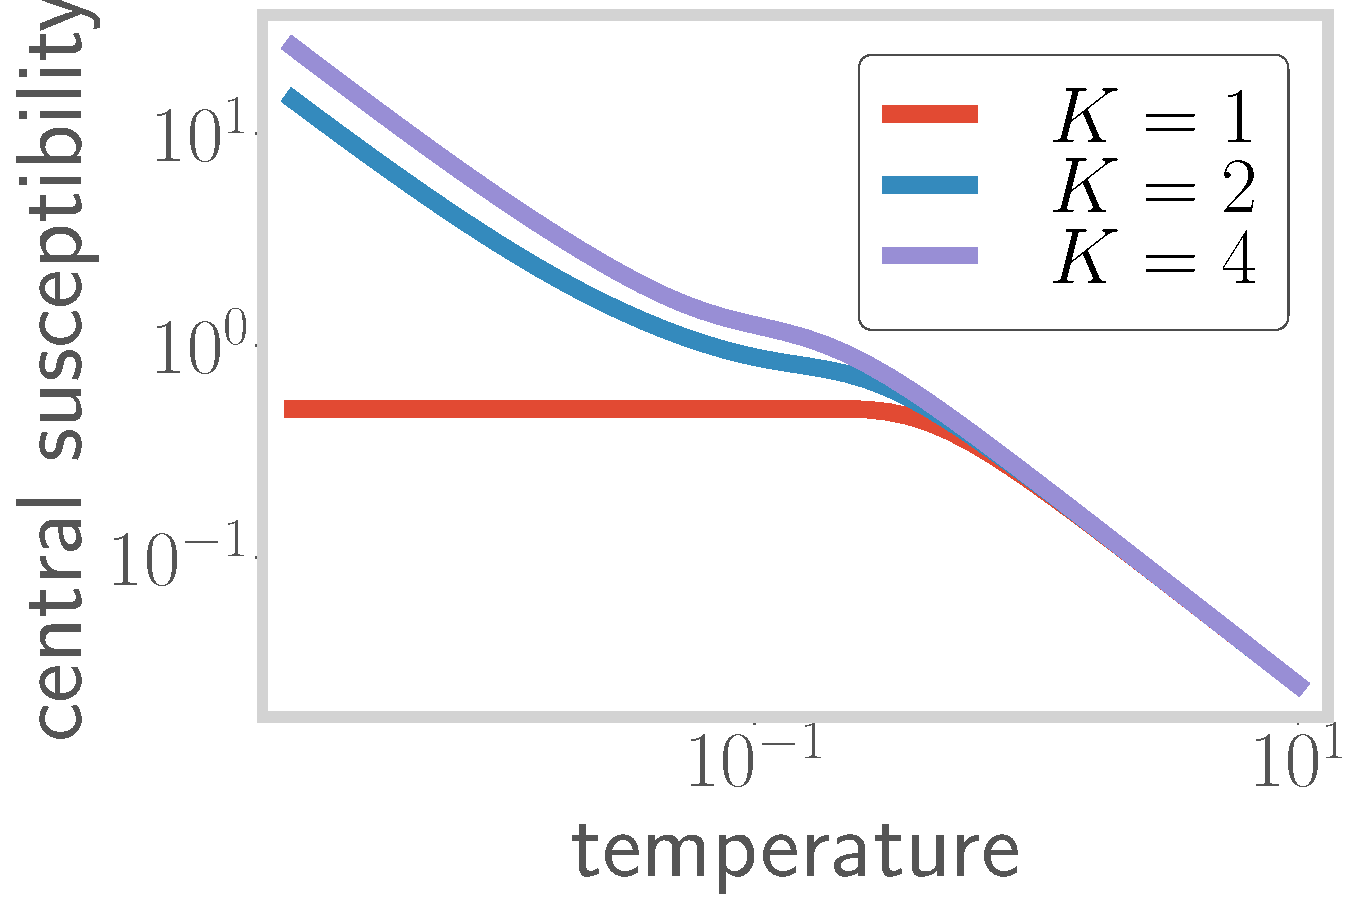
\includegraphics[width=\textwidth]{MCK_imp_chi.pdf}
\end{minipage}

%\hspace*{\fill}
%\begin{minipage}{0.25\textwidth}
%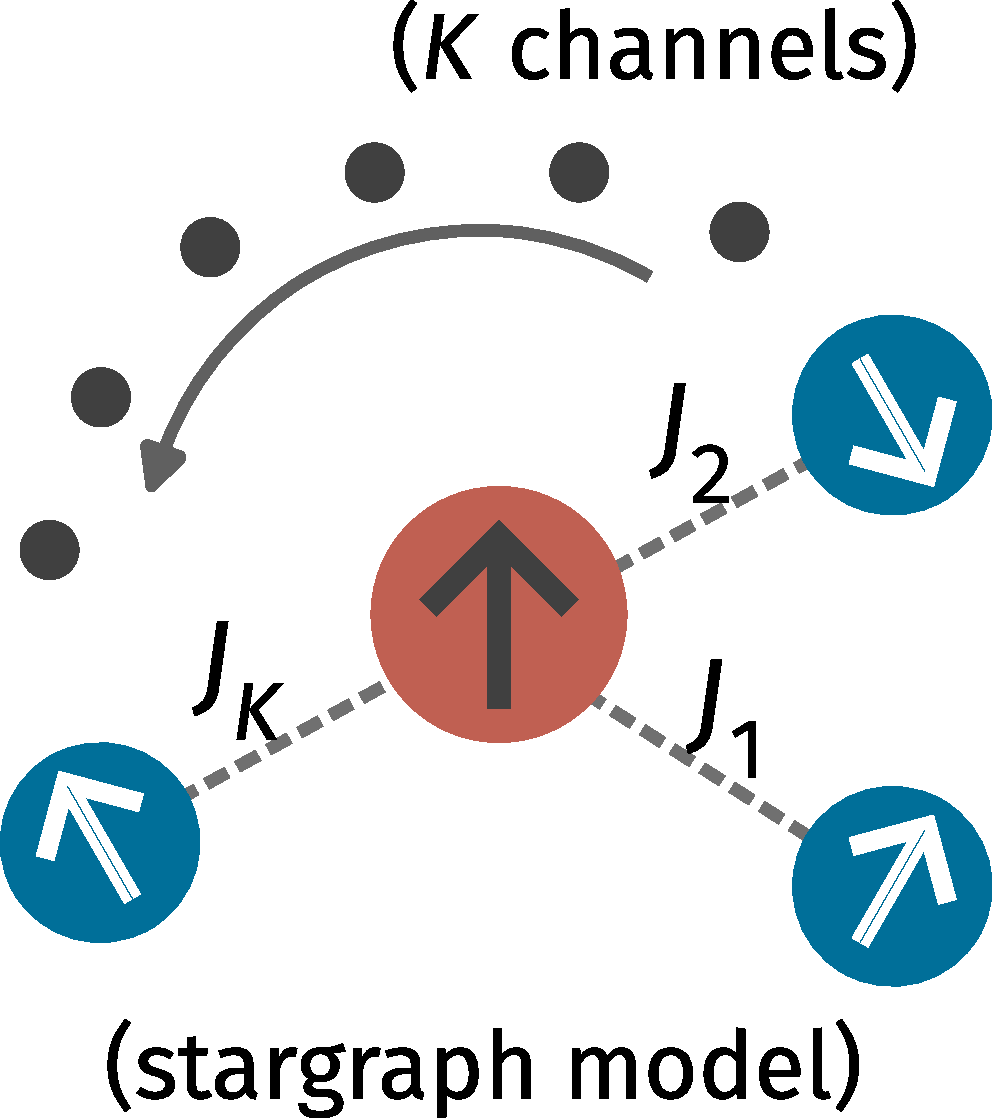
\includegraphics[width=\textwidth]{stargraph.pdf}
%\end{minipage}
%
%\begin{frame}{Can a simpler model make this more intuitive?}
%\footcite{Patra_2023}
%\only<1>{
%\begin{minipage}{0.45\textwidth}
%At \(T=0\) and in the ground state, consider \alert{only} lowest energy state in bath.
%\end{minipage}
%\hspace*{\fill}
%\begin{minipage}{0.45\textwidth}
%	\[KE_\text{bath} + \sum_{l=1}^K J_l \vec{S}_\text{imp}\cdot\vec{s}^{(l)} \Longrightarrow \sum_{l=1}^K J_l \vec{S}_\text{imp}\cdot\vec{s_0}^{(l)} \]
%\end{minipage}
%
%\vspace*{\fill}
%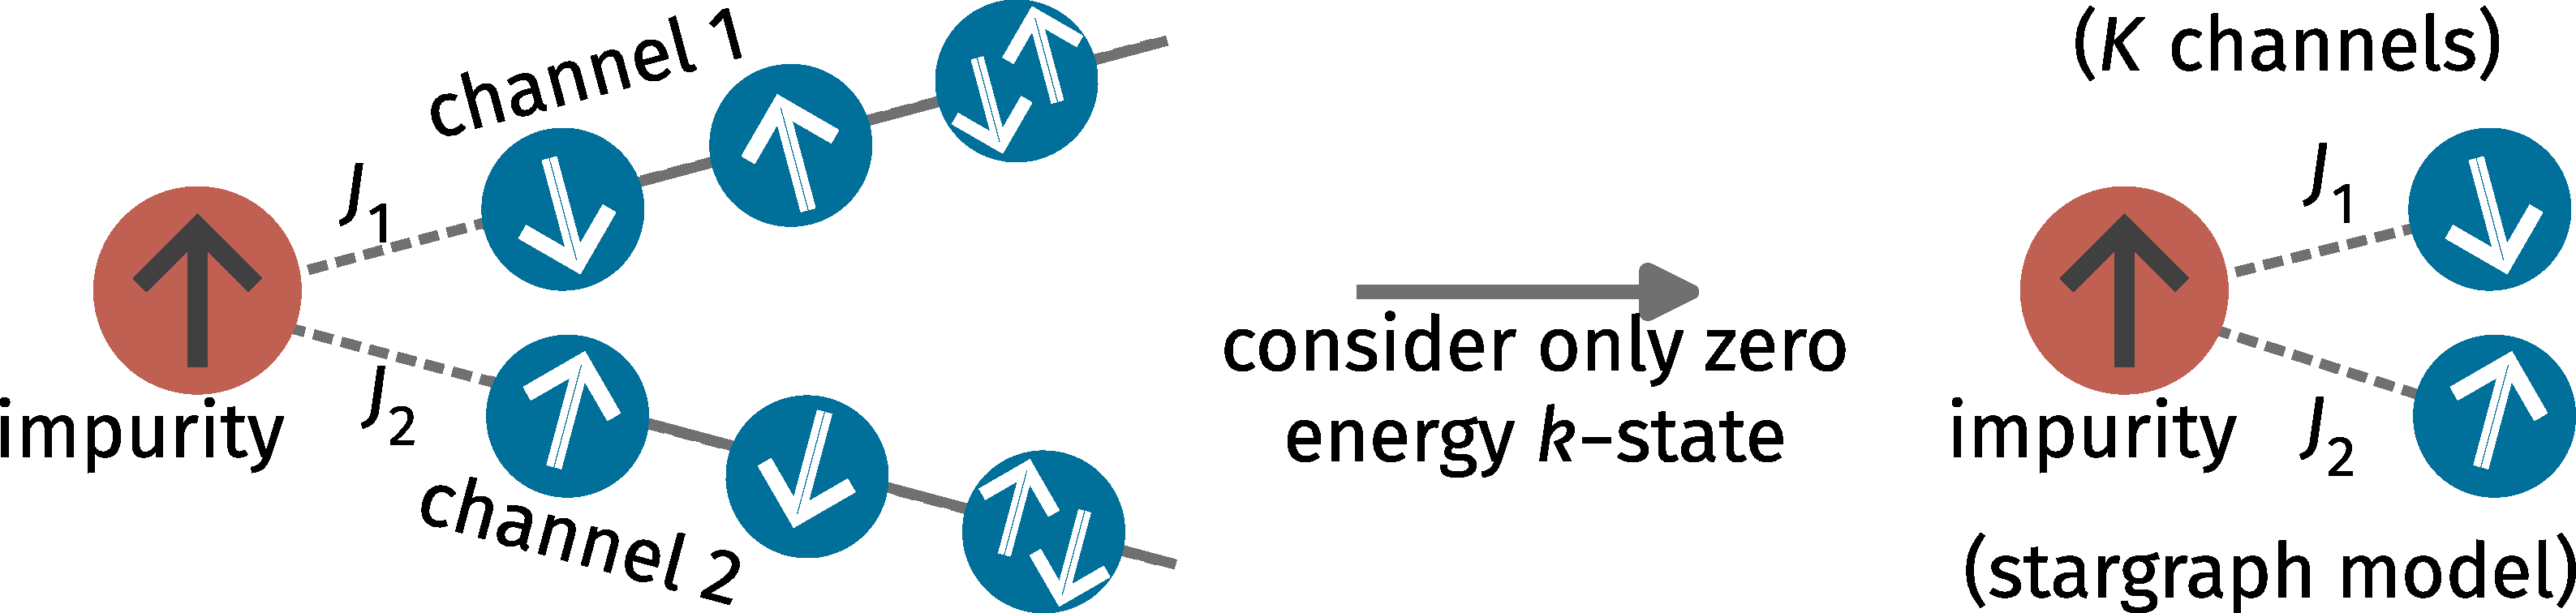
\includegraphics[width=0.7\textwidth]{MCKM_zeroB.pdf}
%}
%\only<2>{
%\begin{minipage}{0.7\textwidth}
%\[\text{Model is (analytically) solvable}: \left\{\ket{S_\text{tot}^z}\right\}\]
%\[\text{Ground state is \alert{degenerate} for $K > 1$}\]
%\begin{itemize}
%	\item Degeneracy for \(K > 1\) shows orthogonality catastrophe\\[10pt]
%	\item \(S_\text{tot}^z \neq 0\) in ground states shows incomplete screening
%\end{itemize}
%\end{minipage}
%\hspace*{\fill}
%\begin{minipage}{0.25\textwidth}
%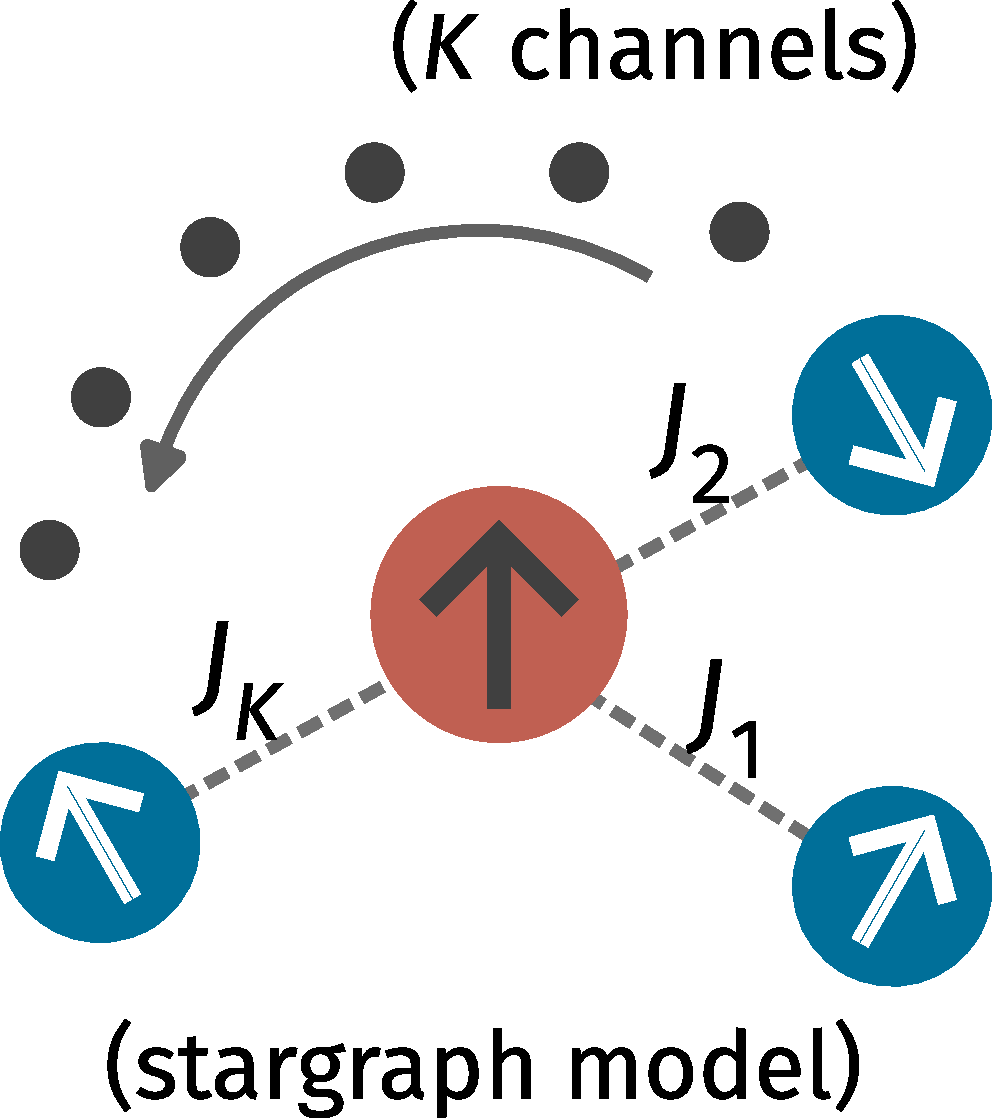
\includegraphics[width=\textwidth]{stargraph.pdf}
%\end{minipage}
%}
%\only<3>{
%\begin{minipage}{0.55\textwidth}
%	Magnetisation of central node goes as 
%	\[ m = \frac{1-K}{2(1 + K)}\]
%\begin{itemize}
%	\item Susceptibility shows \(T=0\) \alert{divergence} for \(K > 1\)\\[10pt]
%	\item Magnetisation can be linked to \alert{scattering phase shifts} and hence to RG equation
%\end{itemize}
%\end{minipage}
%\hspace*{\fill}
%\begin{minipage}{0.35\textwidth}
%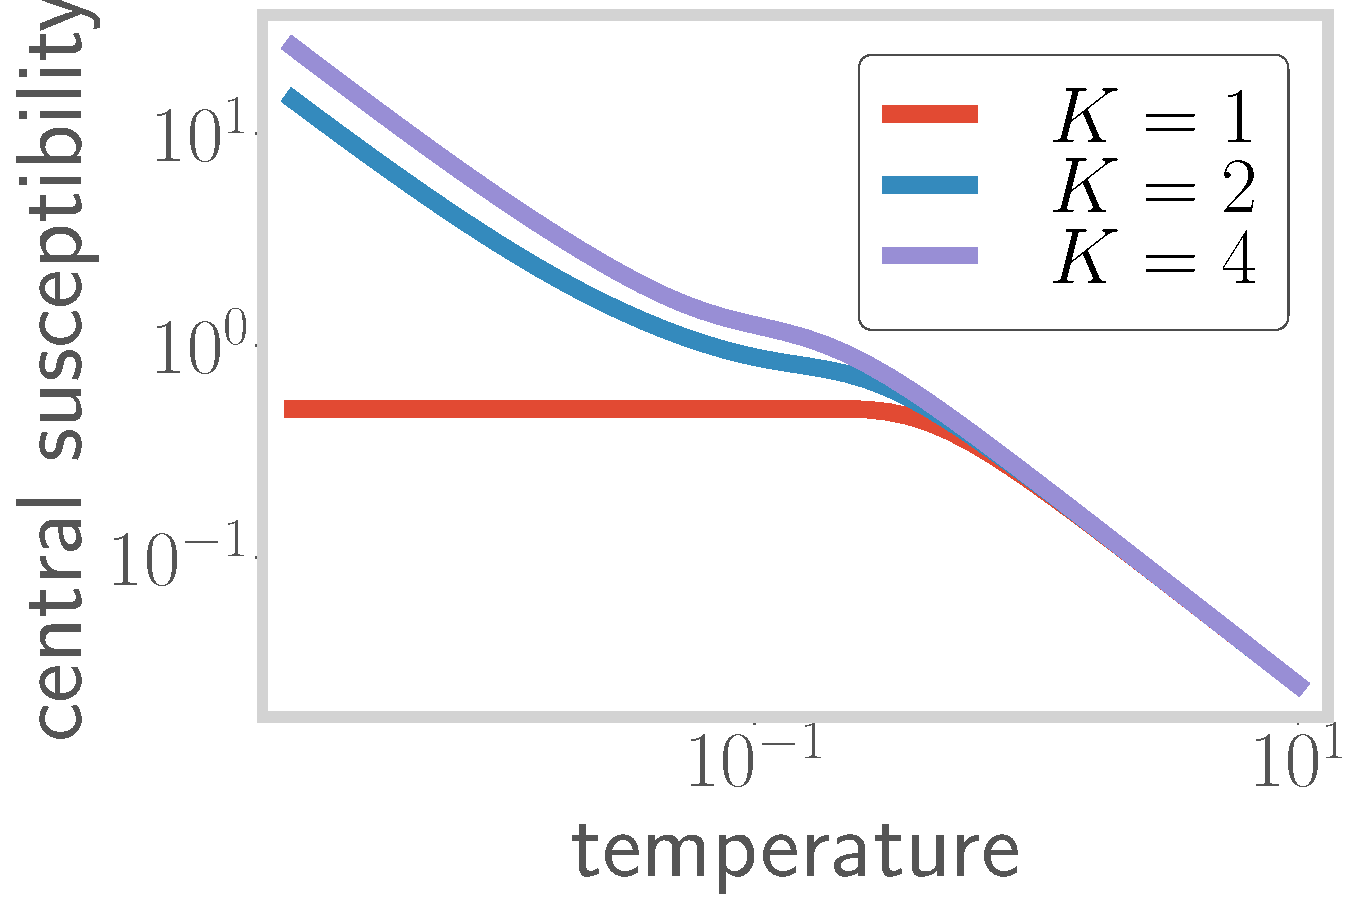
\includegraphics[width=\textwidth]{MCK_imp_chi.pdf}
%\end{minipage}
%}
%\only<4>{
%\begin{minipage}{0.4\textwidth}
%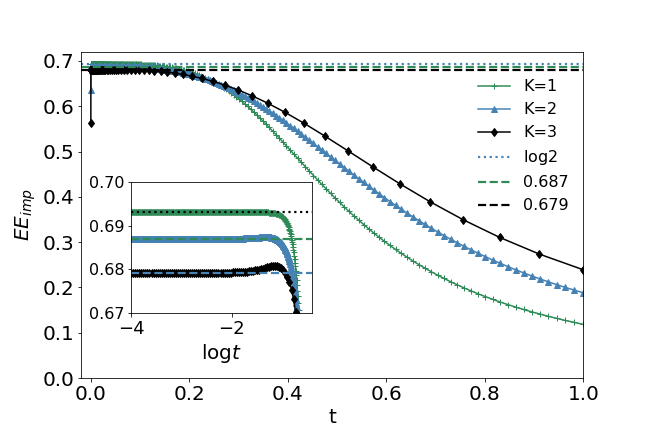
\includegraphics[width=\textwidth]{EE_excitations.png}
%\end{minipage}
%\hspace*{\fill}
%\begin{minipage}{0.55\textwidth}
%Upon including excitations above the stargraph\\
%\begin{itemize}
%	\item entanglement entropy of central node shows \alert{discontinuity} \(\Longrightarrow\) orthogonality catastrophe\\[10pt]
%	\item effective Hamiltonian for these excitations shows \alert{non-Fermi liquid} physics
%\end{itemize}
%\end{minipage}
%}
\end{frame}

\section{How to destroy the Kondo cloud:\\
Effect of local interactions in the bath\vspace*{20pt}}
\begin{textblock*}{\textwidth}(1cm, 3.5cm)

\includegraphics[width=0.9\textwidth]{esiam_arxiv.pdf}\\
\end{textblock*}
\subsection{~}

\begin{frame}{What is the new physics ingredient?}
\footcite{kotliar1992}
\begin{minipage}{0.39\textwidth}
	Add \alert{local correlation} on bath (zeroth) site coupled to impurity
\[KE_\text{bath} + J \vec{S}_\text{imp}\cdot\vec{S}_\text{bath} - U_b\left( \vec{S}_\text{bath} \right)^2 \]
\end{minipage}
\hspace*{\fill}
\begin{minipage}{0.55\textwidth}
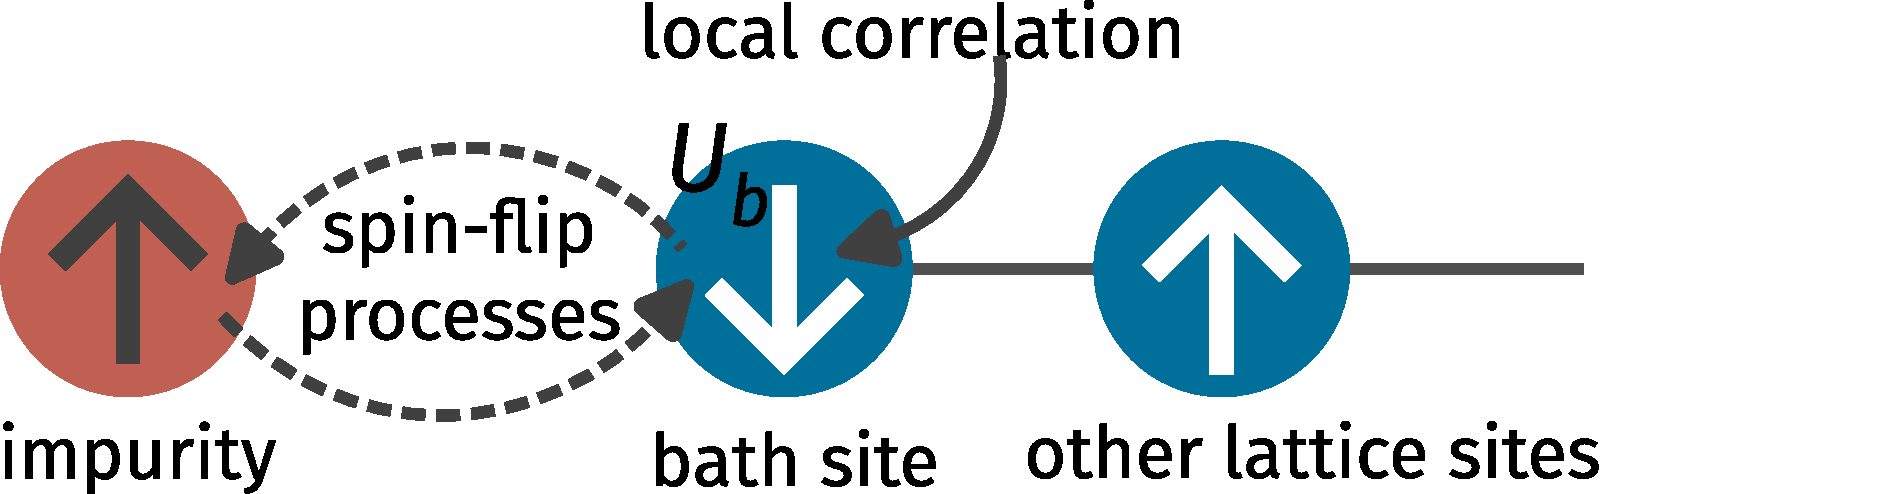
\includegraphics[width=\textwidth]{zeromode_bare.pdf}
\end{minipage}

\vspace*{\fill}
URG equations show that an \alert{attractive} \(U_b\) frustrates the zeroth site.
\[\Delta J \sim J^2 + 4U_b J \implies \text{\alert{phase transition} at }J = -4U_b\]

\vspace*{\fill}
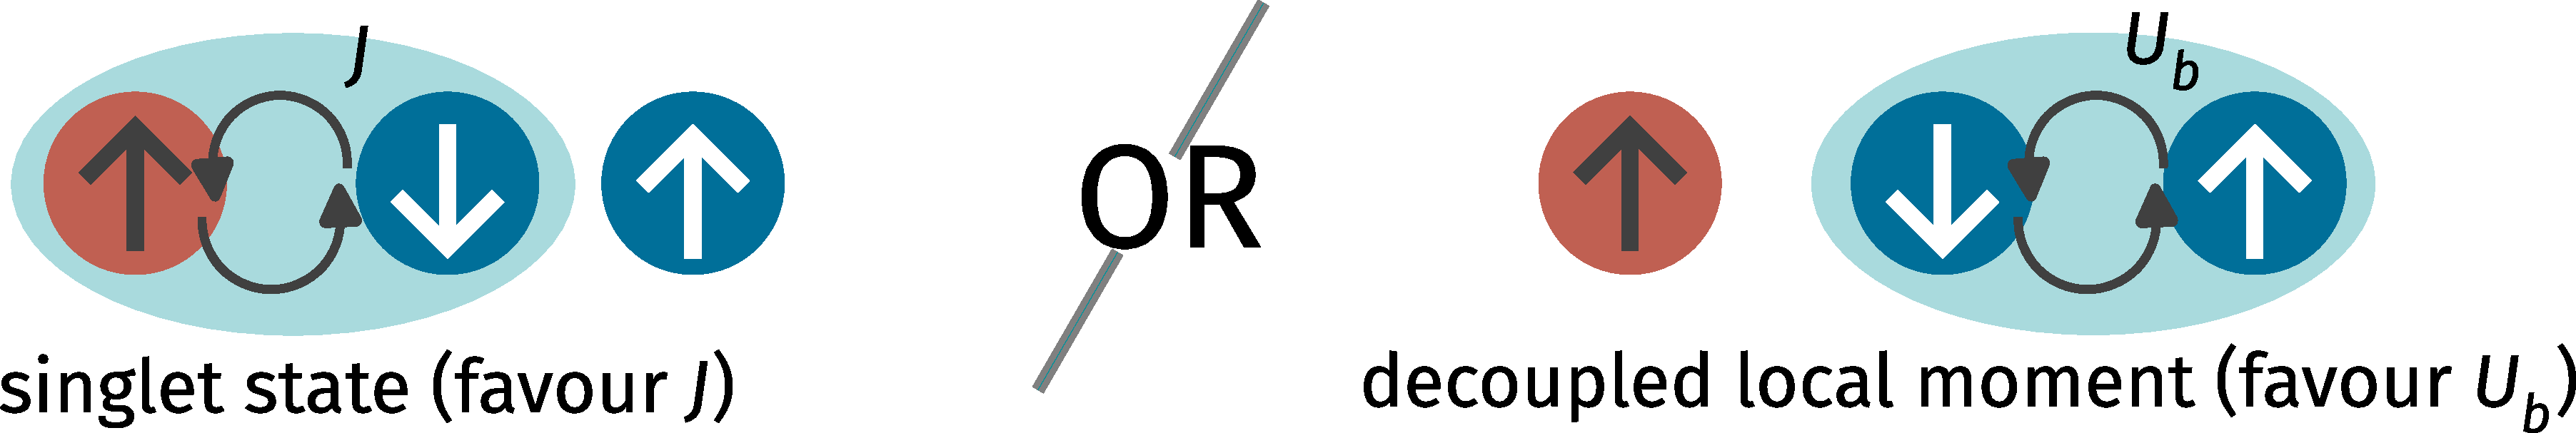
\includegraphics[width=0.9\textwidth]{frustration.pdf}\\

\vspace*{\fill}
Such a model sheds light on the Mott MIT in \(\infty-\)dimensions (as seen from DMFT).
\end{frame}

\begin{frame}{Nature of the transition}
\begin{minipage}{0.45\textwidth}
Across the transition,\\
\begin{itemize}
	\item impurity correlations vanish
	\item bath correlations become non-zero\\[10pt]
\end{itemize}

Shows that \alert{pairing correlations} in the bath are responsible for the transition.
\end{minipage}
\hspace*{\fill}
\begin{minipage}{0.5\textwidth}
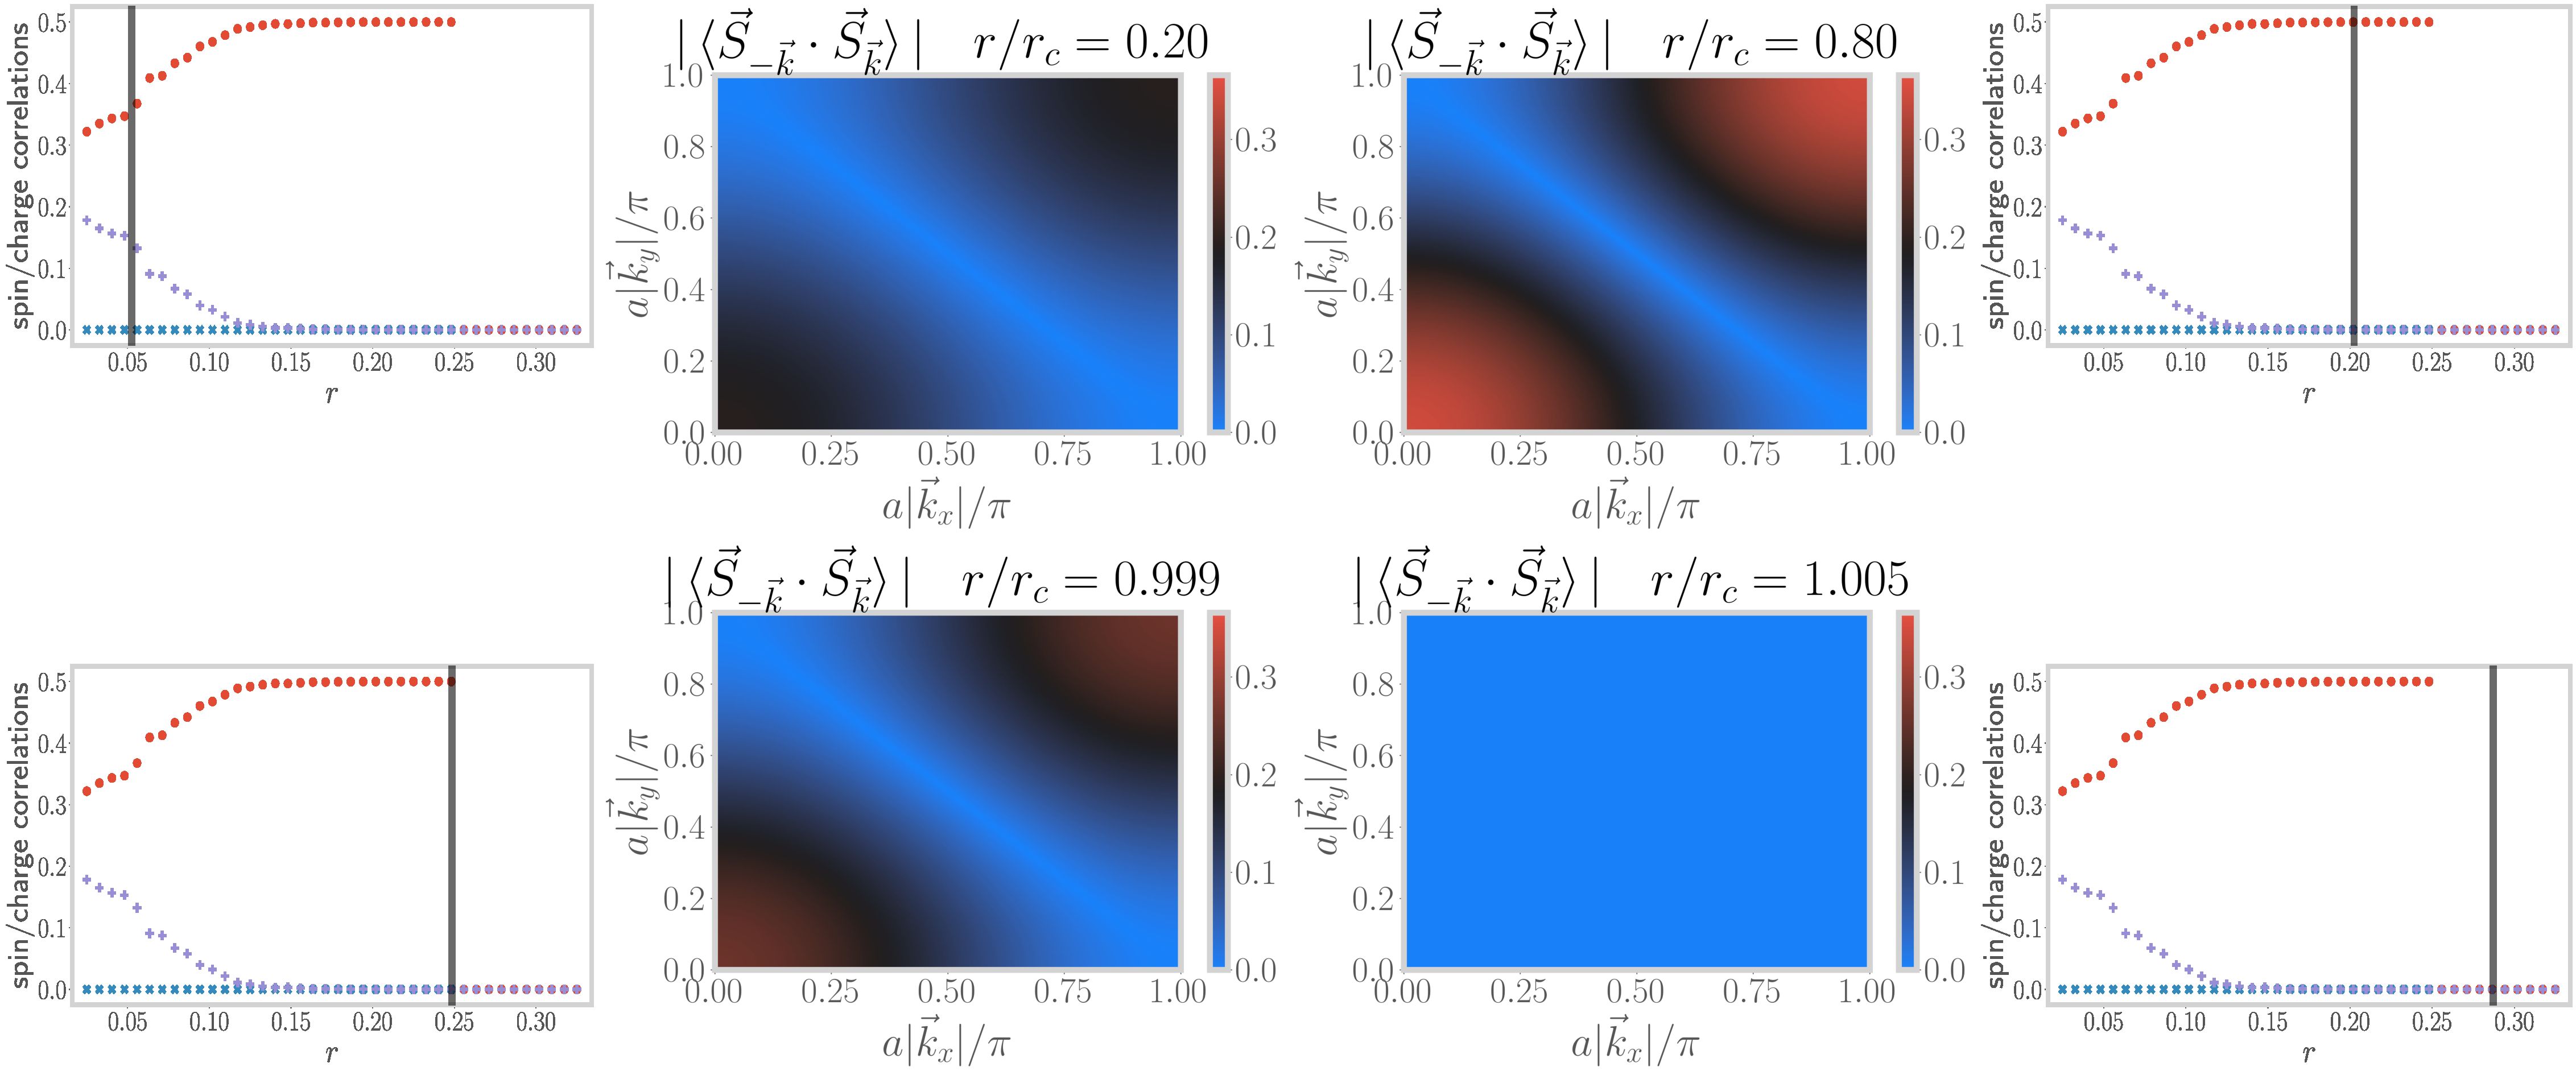
\includegraphics[width=\textwidth]{spin-charge-corr-full.pdf}
\end{minipage}

\vspace*{\fill}
The state \alert{precisely at the transition} is special:
\begin{itemize}
	\item non-Fermi liquid excitations
	\item \alert{fractional} impurity magnetisation and occupancy
\end{itemize}
\end{frame}

\section{Concluding remarks}
\subsection{~}

\begin{frame}{}
	\begin{itemize}
	\item Our analyses often link entanglement measures with correlations, providing bridges between the worlds of condensed matter and quantum information.\\[10pt]
	\item Models of Kondo breakdown can be used to study the effects of measurement on a system coupled to a bath.\\[10pt]
	\begin{center}
	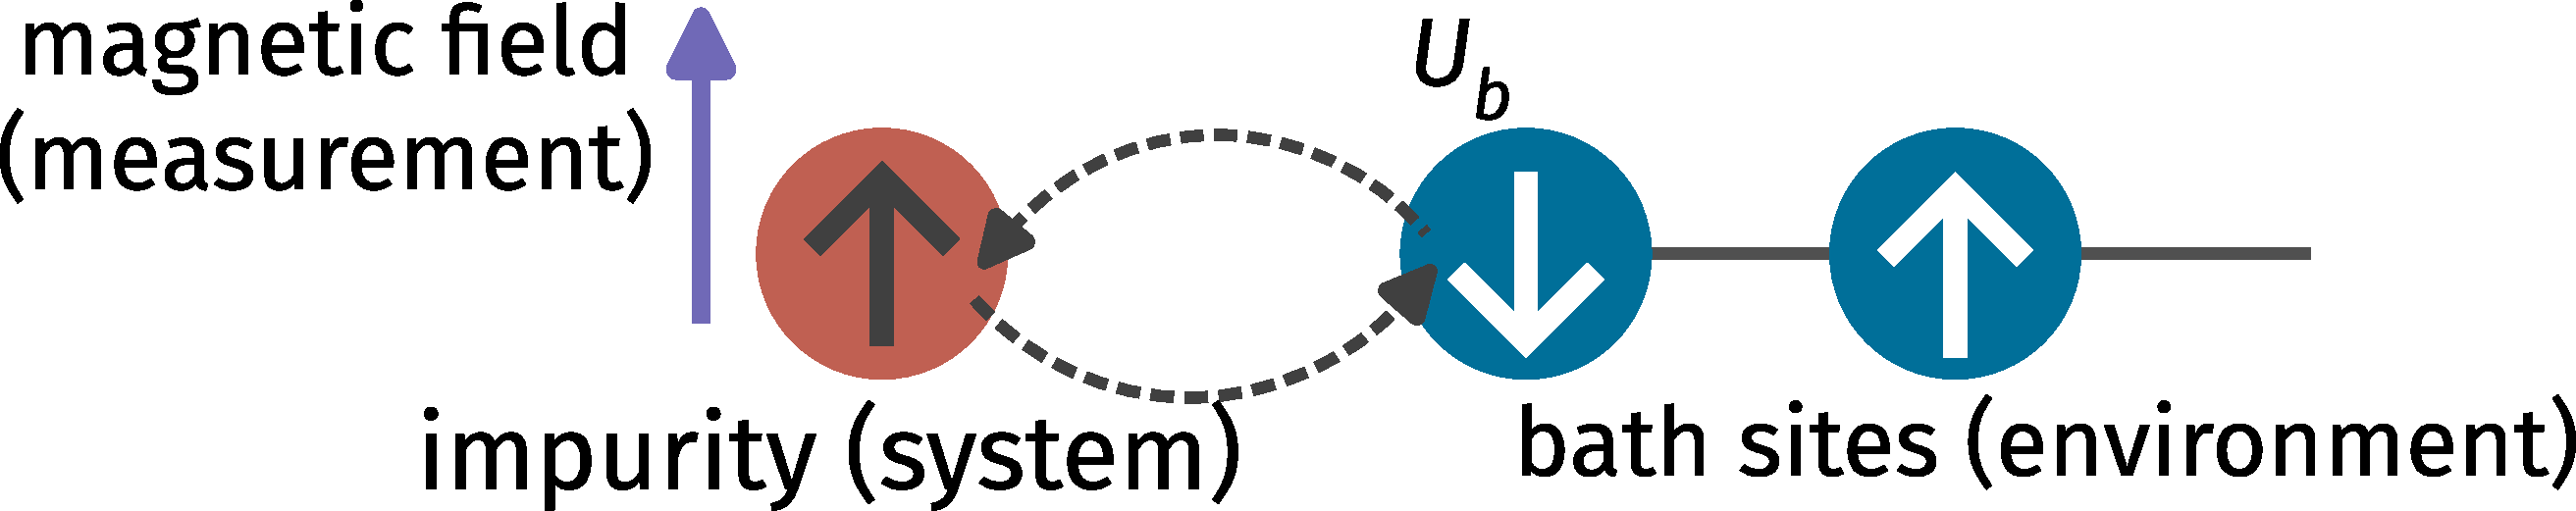
\includegraphics[width=0.5\textwidth]{measurement.pdf}
	\end{center}
	\item The Kondo model with attractive \(U_b\) term has applications in studying the physics of Mott transitions.
\end{itemize}
\end{frame}

\begin{frame}
	
\includegraphics[width=0.65\textwidth]{thanks.pdf}
\end{frame}

\begin{frame}{How to explain the resistance minimum \& eventual saturation?}
\footcite{kondo1964resistance}
\begin{minipage}{0.5\textwidth}
Second order perturbation theory in \(J\) gives:
\[\hspace*{-80pt}\rho \sim T^n - \ln T\]
Explains the \alert{non-monotonic}\\
behaviour!\\[20pt]
However, solution \alert{diverges} at \(T \to 0\)!
\end{minipage}
\begin{minipage}{0.4\textwidth}
	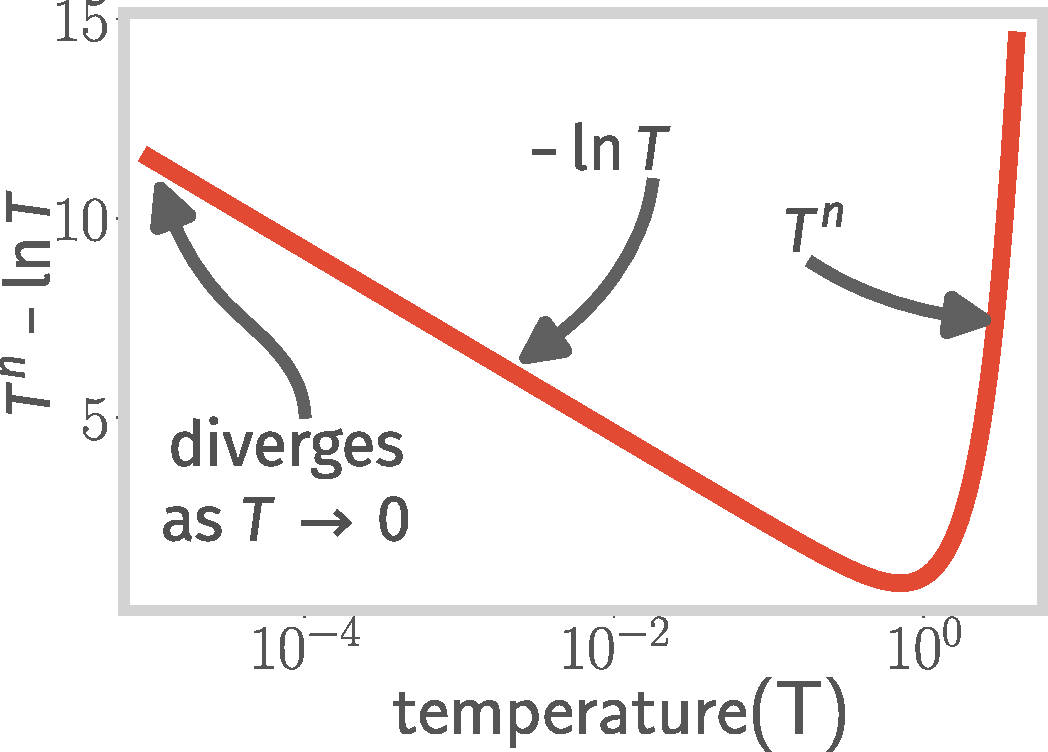
\includegraphics[width=\textwidth]{secondorder.pdf}
\end{minipage}
\begin{textblock*}{0.13\textwidth}(6.5cm, 3.8cm)
	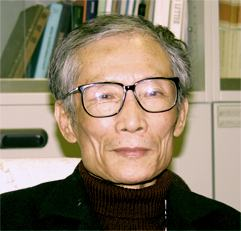
\includegraphics[width=\textwidth]{kondo.jpg}\\
	\footnotesize{(Jun Kondo)}
\end{textblock*}
\end{frame}


\begin{frame}{Unitary RG approach to impurity models}
\footcite{anirbanurg1,anirbanurg2}
\begin{minipage}{0.5\textwidth}
\begin{itemize}
	\item Integrate out \alert{high energy fluctuations} to reach strong-coupling low-energy theory\\[10pt]
	\item Leads to \alert{singlet ground state} and decoupled high-energy \(k-\)states\\[10pt]
	\item Decoupling is carried out through \alert{unitary transformations}
\end{itemize}

\end{minipage}
\hspace*{\fill}
\begin{minipage}{0.4\textwidth}
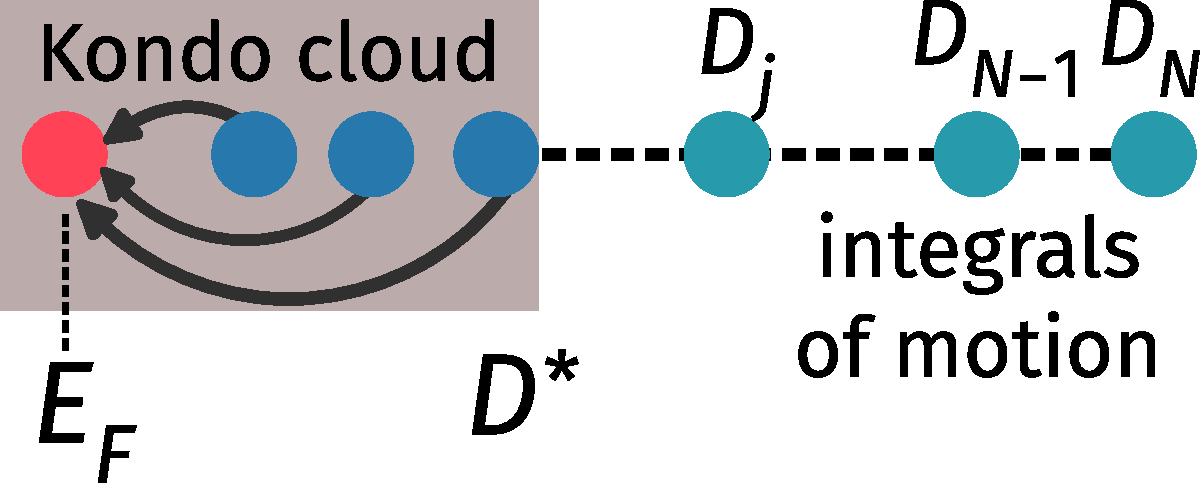
\includegraphics[width=\textwidth]{kondo_fp_1D.pdf}
\end{minipage}
	
\end{frame}

\begin{frame}
\begin{minipage}{0.8\textwidth}
\end{minipage}

\vspace*{\fill}
\begin{itemize}[<+->]
	\item Entanglement entropy \(S(A)\) \(\Longrightarrow\) quantifies how much \alert{information is gained} about the rest of the system by measuring \(A\)\\
	\vspace*{\fill}
	{\centering
	\only<1>{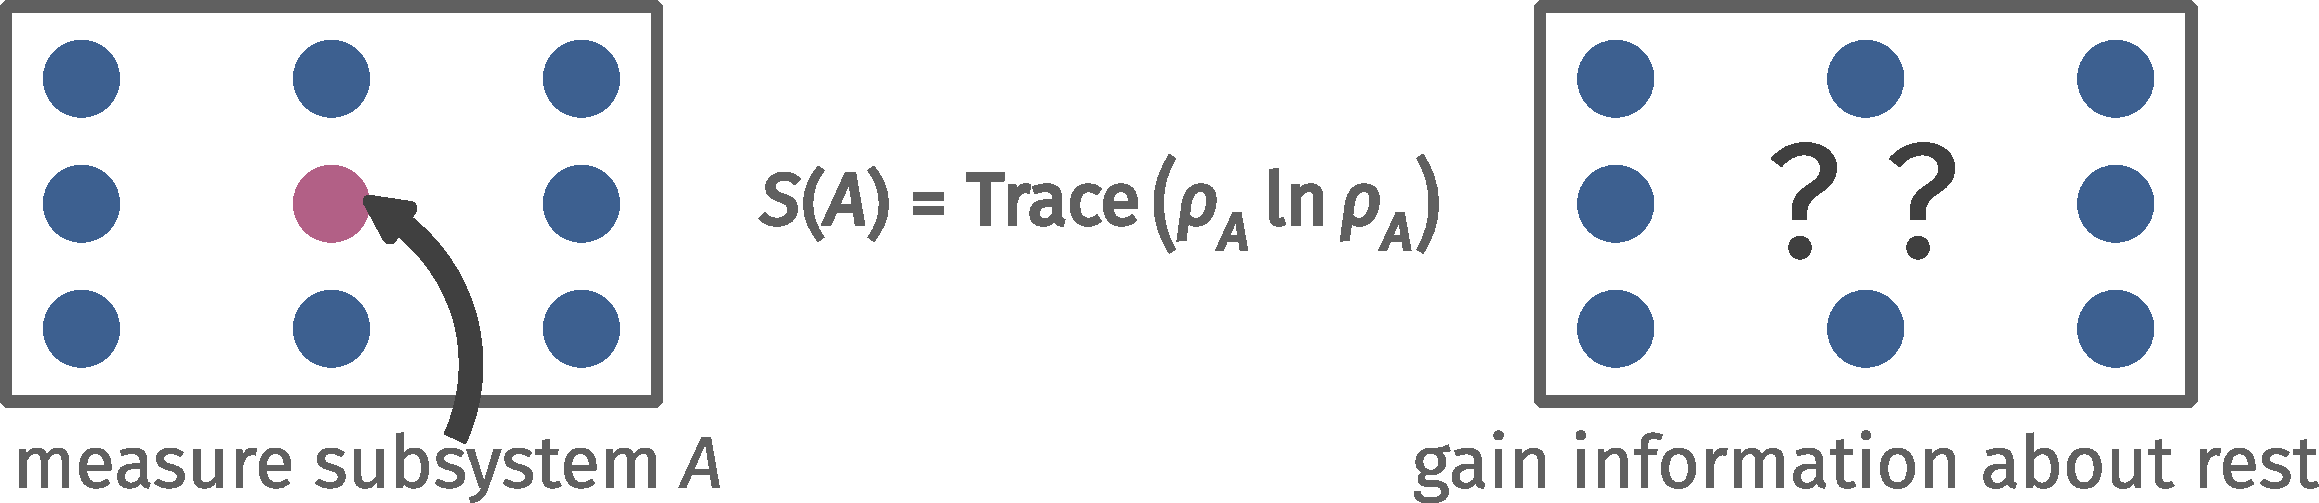
\includegraphics[width=0.85\textwidth]{entanglement.pdf}}}
\item Mutual information \(I_2(A:B)\)\(\Longrightarrow\) quantifies how much \alert{information about subsystem A} is gained by measuring \(B\)\\
	\vspace*{\fill}
	{\centering
	\only<2>{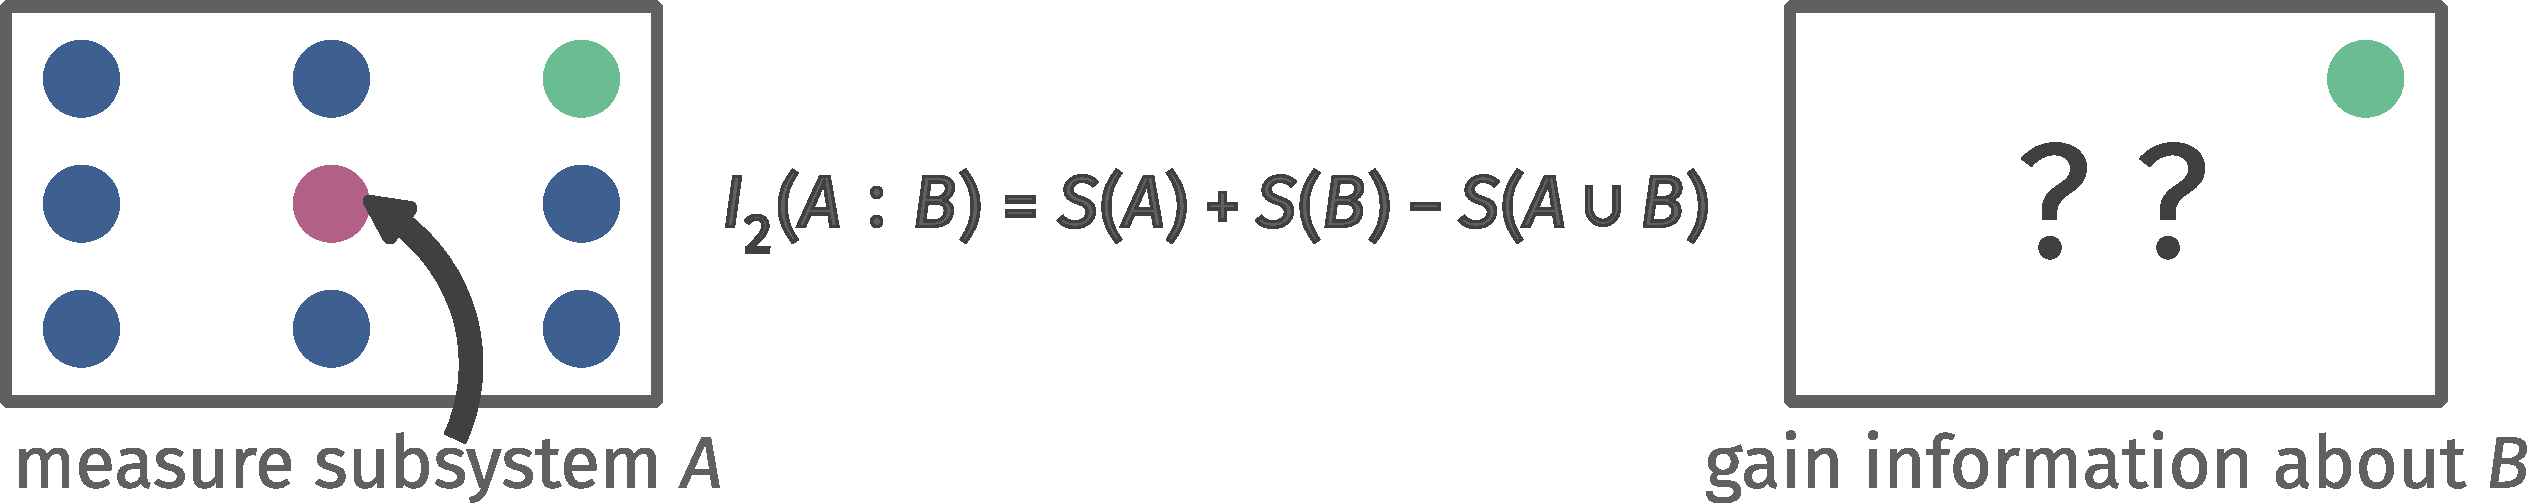
\includegraphics[width=0.85\textwidth]{mutinfo.pdf}}}
\end{itemize}
\end{frame}
\end{document}
